% Options for packages loaded elsewhere
\PassOptionsToPackage{unicode}{hyperref}
\PassOptionsToPackage{hyphens}{url}
\documentclass[
  11pt,
]{article}
\usepackage{xcolor}
\usepackage[margin=1in]{geometry}
\usepackage{amsmath,amssymb}
\setcounter{secnumdepth}{-\maxdimen} % remove section numbering
\usepackage{iftex}
\ifPDFTeX
  \usepackage[T1]{fontenc}
  \usepackage[utf8]{inputenc}
  \usepackage{textcomp} % provide euro and other symbols
\else % if luatex or xetex
  \usepackage{unicode-math} % this also loads fontspec
  \defaultfontfeatures{Scale=MatchLowercase}
  \defaultfontfeatures[\rmfamily]{Ligatures=TeX,Scale=1}
\fi
\usepackage{lmodern}
\ifPDFTeX\else
  % xetex/luatex font selection
\fi
% Use upquote if available, for straight quotes in verbatim environments
\IfFileExists{upquote.sty}{\usepackage{upquote}}{}
\IfFileExists{microtype.sty}{% use microtype if available
  \usepackage[]{microtype}
  \UseMicrotypeSet[protrusion]{basicmath} % disable protrusion for tt fonts
}{}
\makeatletter
\@ifundefined{KOMAClassName}{% if non-KOMA class
  \IfFileExists{parskip.sty}{%
    \usepackage{parskip}
  }{% else
    \setlength{\parindent}{0pt}
    \setlength{\parskip}{6pt plus 2pt minus 1pt}}
}{% if KOMA class
  \KOMAoptions{parskip=half}}
\makeatother
\usepackage{listings}
\newcommand{\passthrough}[1]{#1}
\lstset{defaultdialect=[5.3]Lua}
\lstset{defaultdialect=[x86masm]Assembler}

% --- custom lstset: enable line breaks and small font for code blocks ---
\lstset{
    basicstyle=\ttfamily\small,
    breaklines=true,
    breakatwhitespace=false,
    breakindent=0pt,
    columns=fullflexible,
    keepspaces=true,
    xleftmargin=2pt,
    xrightmargin=2pt,
    frame=single,
    framesep=4pt,
    rulesep=0pt
}
% -----------------------------------------------------------------------

\usepackage{longtable,booktabs,array}
\newcounter{none} % for unnumbered tables
\usepackage{calc} % for calculating minipage widths
% Correct order of tables after \paragraph or \subparagraph
\usepackage{etoolbox}
\makeatletter
\patchcmd\longtable{\par}{\if@noskipsec\mbox{}\fi\par}{}{}
\makeatother
% Allow footnotes in longtable head/foot
\IfFileExists{footnotehyper.sty}{\usepackage{footnotehyper}}{\usepackage{footnote}}
\makesavenoteenv{longtable}
\usepackage{graphicx}
\makeatletter
\newsavebox\pandoc@box
\newcommand*\pandocbounded[1]{% scales image to fit in text height/width
  \sbox\pandoc@box{#1}%
  \Gscale@div\@tempa{\textheight}{\dimexpr\ht\pandoc@box+\dp\pandoc@box\relax}%
  \Gscale@div\@tempb{\linewidth}{\wd\pandoc@box}%
  \ifdim\@tempb\p@<\@tempa\p@\let\@tempa\@tempb\fi% select the smaller of both
  \ifdim\@tempa\p@<\p@\scalebox{\@tempa}{\usebox\pandoc@box}%
  \else\usebox{\pandoc@box}%
  \fi%
}
% Set default figure placement to htbp
\def\fps@figure{htbp}
\makeatother
\setlength{\emergencystretch}{3em} % prevent overfull lines
\providecommand{\tightlist}{%
  \setlength{\itemsep}{0pt}\setlength{\parskip}{0pt}}
\usepackage{bookmark}
\IfFileExists{xurl.sty}{\usepackage{xurl}}{} % add URL line breaks if available
\urlstyle{same}
\hypersetup{
  hidelinks,
  pdfcreator={LaTeX via pandoc}}

\author{}
\date{}

\begin{document}

\section{Dementia Risk Prediction with the SurvivEHR Foundation Model on
UK Biobank Linked Primary Care + Hospital
Data}\label{dementia-risk-prediction-with-the-survivehr-foundation-model-on-uk-biobank-linked-primary-care-hospital-data}

\subsection{Progress Report}\label{progress-report}

\textbf{Cohort}: UK Biobank linked GP primary-care + HES hospital
records (n = 133,322) \textbf{Report date}: 2026-05-15

\begin{center}\rule{0.5\linewidth}{0.5pt}\end{center}

\subsection{1. Executive Summary}\label{executive-summary}

We are building a competing-risk dementia prediction model on UK
Biobank--linked \textbf{GP primary-care records} (Read v2 / CTV3,
\textasciitilde133K cohort patients) and \textbf{HES hospital records}
(ICD-10). The model uses the \textbf{SurvivEHR architecture} (Gadd et
al., 2025, medRxiv) --- a GPT-style transformer foundation-model for EHR
time-to-event prediction --- pretrained on our local UKB GP records and
fine-tuned for dementia. It outputs a full \textbf{25-year cumulative
incidence function (CIF)} for both dementia and competing death via a
DeSurv ODE head.

The two strongest results on the canonical 8,241-patient test cohort are
summarised below. Neither model wins every metric: \textbf{Single-GP +
HESstatic} is best on top-1\% PPV (clinical screening yield) and on
dementia IBS calibration; \textbf{Dual + HESstatic + SST1\%} is best on
time-dependent C-index (overall discrimination) and on broader-cut PPV
(top 5\%).

{\def\LTcaptype{none} % do not increment counter
\begin{longtable}[]{|>{\raggedright\arraybackslash}p{(\linewidth - 4\tabcolsep) * \real{0.3333}}|>{\raggedright\arraybackslash}p{(\linewidth - 4\tabcolsep) * \real{0.3333}}|>{\raggedright\arraybackslash}p{(\linewidth - 4\tabcolsep) * \real{0.3333}}|}
\hline
\begin{minipage}[b]{\linewidth}\raggedright
Metric (5-year horizon)
\end{minipage} & \begin{minipage}[b]{\linewidth}\raggedright
Single-GP + HESstatic \emph{(clean baseline; best top-1\% PPV, best IBS
dem)}
\end{minipage} & \begin{minipage}[b]{\linewidth}\raggedright
Dual (GP+HES) + HESstatic + 1\% SST \emph{(best C-index, best PPV@5\%)}
\end{minipage} \\
\hline
\hline
\endhead
\hline
\endlastfoot
Time-dependent C-index (Antolini), dementia & 0.8451 &
\textbf{0.8506} \\
\hline
C-index, death & \textbf{0.9622} & 0.9589 \\
\hline
Integrated Brier Score, dementia (lower = better) & \textbf{0.3152} &
0.3265 \\
\hline
5-year AUROC (binary, exclude\_early\_censored) & 0.9236 &
\textbf{0.9271} \\
\hline
5-year PPV @ top 1\% / 5\% / 10\% & \textbf{68.9\%} / 27.9\% / 19.0\% &
55.6\% / \textbf{29.7\%} / 19.3\% \\
\hline
\end{longtable}
}

For external context, the most directly comparable foundation-model EHR
paper, \textbf{TRADE} (Wisnivesky et al., NYU AD/ADRD/MCI prediction),
reports 5y AUROC = 0.735 and PPV@top 1\% = 39.2\%. Detailed code-set
overlap analysis (§8) confirms our HES dementia label is a near-strict
subset of TRADE's umbrella, with the main gaps being MCI (no UK ICD-10
equivalent) and FTD/Lewy body sub-codes (\textasciitilde160 extra
patients available if we extend our label).

\begin{center}\rule{0.5\linewidth}{0.5pt}\end{center}

\subsection{2. Data Sources}\label{data-sources}

\subsubsection{2.1 The two data sources}\label{the-two-data-sources}

We use \textbf{two UK Biobank--linked sources}:

\begin{enumerate}
\def\labelenumi{\arabic{enumi}.}
\tightlist
\item
  \textbf{UKB-linked GP primary-care extract} --- General Practice
  records (Read v2 / CTV3 clinical coding) covering 502,246 UKB
  participants in total (of which 230,001 have ≥1 diagnostic record).
  Contains the full longitudinal record of GP encounters: diagnoses,
  prescriptions, lab tests, lifestyle observations, referrals, and
  administrative events.
\item
  \textbf{UKB-linked HES (Hospital Episode Statistics)} ---
  Secondary-care records (ICD-10 diagnoses, OPCS-4 procedures) covering
  448,985 UKB participants. Contains admission dates, primary/secondary
  diagnosis lists, and operation lists.
\end{enumerate}

The two sources are linked at the patient level via UKB's encrypted
participant ID.

\subsubsection{2.2 GP primary-care record is NOT just
diagnoses}\label{gp-primary-care-record-is-not-just-diagnoses}

A common misunderstanding is that GP records contain only diagnosis
codes. In reality, the Read v2 vocabulary used in UK GP systems contains
\textbf{108,118 distinct tokens} in our pretrained model's vocabulary,
spanning a wide range of clinical event types.

Read v2 uses semantic prefixes to group code categories. The main
chapters are roughly:

{\def\LTcaptype{none} % do not increment counter
\begin{longtable}[]{|>{\raggedright\arraybackslash}p{(\linewidth - 2\tabcolsep) * \real{0.5000}}|>{\raggedright\arraybackslash}p{(\linewidth - 2\tabcolsep) * \real{0.5000}}|}
\hline
\begin{minipage}[b]{\linewidth}\raggedright
Chapter prefix
\end{minipage} & \begin{minipage}[b]{\linewidth}\raggedright
Category
\end{minipage} \\
\hline
\hline
\endhead
\hline
\endlastfoot
\passthrough{\lstinline!1...!} & History and process codes (symptoms,
presenting complaint) \\
\hline
\passthrough{\lstinline!2...!} & Examination findings, physical
measurements (BP, weight, BMI) \\
\hline
\passthrough{\lstinline!3...!} & Diagnostic procedures (ECG, imaging) \\
\hline
\passthrough{\lstinline!4...!} & Laboratory tests (blood, urine,
etc.) \\
\hline
\passthrough{\lstinline!6...!} & Administrative / preventive (screening,
counselling) \\
\hline
\passthrough{\lstinline!8...!} & Other procedures (vaccinations, minor
surgery) \\
\hline
\passthrough{\lstinline!9...!} & Administrative (letters, referrals,
registrations) \\
\hline
\passthrough{\lstinline!B...!} & Neoplasms \\
\hline
\passthrough{\lstinline!E...!} & Mental disorders \\
\hline
\passthrough{\lstinline!F...!} & Nervous system (incl.~dementia) \\
\hline
\passthrough{\lstinline!G...!} & Circulatory (cardiovascular) \\
\hline
\passthrough{\lstinline!H...!} & Respiratory \\
\hline
\passthrough{\lstinline!J...!} & Digestive \\
\hline
\passthrough{\lstinline!K...!} & Genitourinary \\
\hline
\passthrough{\lstinline!Eu0..!} & ICD-10 mapped mental disorders
(incl.~dementia F00-F09) \\
\hline
\end{longtable}
}

So in the GP record stream one can see: a diagnostic code (e.g.,
\passthrough{\lstinline!G20..!} essential hypertension), then a blood
test result (\passthrough{\lstinline!44..!} cholesterol), then a
prescription, then a referral letter (\passthrough{\lstinline!9..!}),
then a measurement (\passthrough{\lstinline!229..!} body weight), etc.
The model sees this \textbf{chronologically ordered stream} of event
codes + dates + numeric values (where applicable), \textbf{not} an
aggregated feature vector.

\textbf{Example patient (anonymised, real record from our test cohort):}

\begin{lstlisting}
PATIENT_ID:    2442387
YEAR_OF_BIRTH: 1941    SEX: M    IMD: 3    ETHNICITY: White British
INDEX_DATE:    2013-01-01 (= 72nd birthday)

Total GP events recorded:      379 events from 1961-01-01 to 2012-12-31
HES pre-index admissions:      4 (HES_TOTAL_ADMISSIONS scaled = 0.279)
HES comorbidity flags:         none of stroke/MI/HF/HT/diabetes etc. set

First 10 GP events (chronological), raw codes:
  1961-01-01   J16y4
  1971-01-01   H51..
  1974-01-01   G20..
  2000-01-01   1241.
  2000-01-01   12C1.
  2000-01-01   12C3.
  2000-01-01   12A1.
  2000-01-01   12C4.
  2002-12-01   G5y34
  2005-08-01   J51..
... (total 379 events; final event determines the patient's outcome label)
\end{lstlisting}

The descriptive labels for each Read v2 code are NOT used by the model
--- the model only sees the raw code tokens. Translation of any specific
code to a description requires a Read v2 dictionary lookup (we have not
embedded such a dictionary in the report, as the model does not rely on
it).

\subsubsection{2.3 Cohort composition}\label{cohort-composition}

{\def\LTcaptype{none} % do not increment counter
\begin{longtable}[]{|>{\raggedright\arraybackslash}p{(\linewidth - 2\tabcolsep) * \real{0.5000}}|>{\raggedright\arraybackslash}p{(\linewidth - 2\tabcolsep) * \real{0.5000}}|}
\hline
\begin{minipage}[b]{\linewidth}\raggedright
Stage
\end{minipage} & \begin{minipage}[b]{\linewidth}\raggedright
Patient count
\end{minipage} \\
\hline
\hline
\endhead
\hline
\endlastfoot
Total UKB-linked GP primary-care database
(\passthrough{\lstinline!static\_table!}, all UKB participants with GP
linkage) & \textbf{502,246} \\
\hline
Of these, with ≥1 diagnostic record in
\passthrough{\lstinline!diagnosis\_table!} & 230,001 \\
\hline
Total UKB-linked HES hospital database & \textbf{448,985} \\
\hline
In BOTH GP and HES (HES is a subset of the GP-linked set) & 448,985 \\
\hline
GP-only (no HES linkage) & 53,261 \\
\hline
Meeting study inclusion (≥1y GP registration, ≥5 events before idx 72,
idx age in 50-90) & \textbf{133,322} \\
\hline
After GP-prevalent dementia leakage removal (cleanest cohort) &
\textbf{133,076} \\
\hline
\end{longtable}
}

\textbf{Dementia capture by data source} (in the full UKB linkage layer,
before applying our cohort filter):

{\def\LTcaptype{none} % do not increment counter
\begin{longtable}[]{|>{\raggedright\arraybackslash}p{(\linewidth - 4\tabcolsep) * \real{0.3333}}|>{\raggedright\arraybackslash}p{(\linewidth - 4\tabcolsep) * \real{0.3333}}|>{\raggedright\arraybackslash}p{(\linewidth - 4\tabcolsep) * \real{0.3333}}|}
\hline
\begin{minipage}[b]{\linewidth}\raggedright
Source
\end{minipage} & \begin{minipage}[b]{\linewidth}\raggedright
Dementia patients
\end{minipage} & \begin{minipage}[b]{\linewidth}\raggedright
Note
\end{minipage} \\
\hline
\hline
\endhead
\hline
\endlastfoot
GP (31 strict Read v2 dementia codes) & \textbf{992} & Formal GP-coded
dementia \\
\hline
HES (F00.\emph{, F01.}, F02.\emph{, F03, G30.}) & \textbf{8,941} &
Hospital ICD-10 dementia \\
\hline
In BOTH GP and HES & 781 & \\
\hline
GP-only & 211 & \\
\hline
HES-only & 8,160 & \textbf{HES catches \textasciitilde9× more dementia
than GP} \\
\hline
\textbf{Total unique (GP ∪ HES)} & \textbf{9,152} & \\
\hline
\end{longtable}
}

\textbf{Key finding}: HES catches \textbf{almost an order of magnitude
more dementia patients than GP}. UK GP records substantially under-code
dementia --- patients are often diagnosed in memory clinics or hospital
admissions (which goes to HES) but the GP record is never updated. This
is consistent with the well-documented 30--50\% GP under-diagnosis rate
(Lang 2017; Connolly 2011) and strongly motivates the self-training
pipeline.

\textbf{Within our 133,322 study cohort} (subset of the 502,246 full
linkage after applying inclusion criteria: idx age 72, ≥1y GP
registration, ≥5 events before index):

{\def\LTcaptype{none} % do not increment counter
\begin{longtable}[]{|>{\raggedright\arraybackslash}p{(\linewidth - 2\tabcolsep) * \real{0.5000}}|>{\raggedright\arraybackslash}p{(\linewidth - 2\tabcolsep) * \real{0.5000}}|}
\hline
\begin{minipage}[b]{\linewidth}\raggedright
Has data in
\end{minipage} & \begin{minipage}[b]{\linewidth}\raggedright
Patients (\% cohort)
\end{minipage} \\
\hline
\hline
\endhead
\hline
\endlastfoot
GP records (all 133,322 must have GP --- inclusion criterion) & 133,322
(100\%) \\
\hline
With ≥1 valid ICD-10 HES record (any time) & 126,530 (94.9\%) \\
\hline
GP-only dementia (31 strict, not in HES) & 162 (0.12\%) \\
\hline
HES-only dementia (not in GP) & 5,477 (4.11\%) \\
\hline
Both GP and HES dementia & 519 (0.39\%) \\
\hline
\textbf{Total dementia patients (GP ∪ HES, ever)} & \textbf{6,158
(4.62\%)} \\
\hline
\end{longtable}
}

The 6,158 within-cohort number is smaller than the 9,152 full-linkage
number because \textbf{the inclusion criteria drop 2,994 dementia
patients} who fail one or more criteria (e.g., do not have a GP visit at
age 72, insufficient GP registration history, or fewer than 5 pre-index
events). The within-cohort prevalence (4.62\%) is approximately 2× the
UK general elderly baseline because we deliberately recruited at age 72.

\subsubsection{2.4 Train / Val / Test split}\label{train-val-test-split}

Splits are made at the \textbf{GP practice level}
(\passthrough{\lstinline!PRACTICE\_ID!}), not at the patient level. All
patients in a given practice go to the same split. This prevents
practice-level data leakage (e.g., regional coding patterns,
practice-specific terminology).

{\def\LTcaptype{none} % do not increment counter
\begin{longtable}[]{|>{\raggedright\arraybackslash}p{(\linewidth - 8\tabcolsep) * \real{0.2000}}|>{\raggedright\arraybackslash}p{(\linewidth - 8\tabcolsep) * \real{0.2000}}|>{\raggedright\arraybackslash}p{(\linewidth - 8\tabcolsep) * \real{0.2000}}|>{\raggedright\arraybackslash}p{(\linewidth - 8\tabcolsep) * \real{0.2000}}|>{\raggedright\arraybackslash}p{(\linewidth - 8\tabcolsep) * \real{0.2000}}|}
\hline
\begin{minipage}[b]{\linewidth}\raggedright
Split
\end{minipage} & \begin{minipage}[b]{\linewidth}\raggedright
Patients
\end{minipage} & \begin{minipage}[b]{\linewidth}\raggedright
Dementia events
\end{minipage} & \begin{minipage}[b]{\linewidth}\raggedright
Death events
\end{minipage} & \begin{minipage}[b]{\linewidth}\raggedright
Censored
\end{minipage} \\
\hline
\hline
\endhead
\hline
\endlastfoot
Train & 119,271 & 5,286 & 7,898 & 106,087 \\
\hline
Val & 5,794 & 296 & 485 & 5,013 \\
\hline
Test & 8,257 & 376 (370 after canonical filter to 8,241) & 451 &
7,430 \\
\hline
\textbf{Total} & \textbf{133,322} & \textbf{5,958} & \textbf{8,834} &
\textbf{118,530} \\
\hline
\end{longtable}
}

Dementia event prevalence across the full cohort = 5,958 / 133,322 =
\textbf{4.47\%}; death prevalence = 6.63\%; censored = 88.91\%. Splits
are approximately stratified by event rate.

(Note: 5,958 incident dementia events vs 6,158 patients with any
dementia code in GP/HES history --- see §2.3 --- differ by
\textasciitilde200. The gap is patients whose dementia code occurs
before the prediction point, or who die from another cause first; these
are not labeled as ``incident dementia event'' in the V2 dataset.)

\textbf{⚠️ Important caveat about train/val/test cleanliness}: The 246
GP-prevalent dementia patients (213 train / 17 val / 16 test) --- i.e.,
patients whose dementia code appears \textbf{before} the prediction
point --- are present in the V2 dataset and were used to train all five
``V2 clean labels'' post-leakage models (Single-GP + HESstatic through
Dual + HESstatic + SST5\%). \textbf{Only the test set is filtered} to
the canonical 8,241 = 8,257 − 16 for evaluation. The ``leakage-fixed''
base dataset that removes all 246 patients is used by the most recent
model \textbf{Single-GP + HESstatic + leak-fix} (§5, §7.1). All
test-cohort metrics in §7.1 are therefore on the same canonical 8,241
patients; training-set leakage of 213+17 = 230 patients (0.18\% of
train+val) was tolerated in the V2-labelled comparison set to keep model
comparisons consistent with our historical experimental record.

\begin{center}\rule{0.5\linewidth}{0.5pt}\end{center}

\subsection{3. Label Definition}\label{label-definition}

\subsubsection{3.1 Index date and prediction setup (important
clarification)}\label{index-date-and-prediction-setup-important-clarification}

The study fixes \textbf{age 72 as the cohort entry date} for inclusion
(all patients must have at least one GP visit at age 72), but this is
\textbf{not the prediction time-point}. The model performs
\textbf{dynamic prediction}:

\begin{lstlisting}
Past:  [........ GP events ........]
                                   ↑
                          Prediction point = the patient's most recent
                          pre-index GP encounter (often months/years BEFORE age 72)

Future: [...]→ dementia / death / censored
        time = days from prediction point (NOT from age 72)
\end{lstlisting}

The model emits CIF over
\passthrough{\lstinline!t = 0 → 25 years from the prediction point!}.
This matches how the model is actually deployed: a clinician asks
``given everything I know about this patient up to today, what is their
risk over the next N years?'' --- not ``what is their risk from a
fictitious cohort entry date.''

The ``index age 72'' is used only for \textbf{inclusion / exclusion},
not for time origin. Events occurring before the prediction point are
model input; events occurring after are target outcomes.

\subsubsection{3.2 Dementia label: GP side (41 Read v2
codes)}\label{dementia-label-gp-side-41-read-v2-codes}

The full list of Read v2 / CTV3 codes used to identify dementia events
on the GP side, with \textbf{patient counts in the raw GP database
(230,001 patients with diagnostic records, drawn from the 502,246
UKB-linked GP cohort)} --- note: these are unique-patient counts, not
event counts.

{\def\LTcaptype{none} % do not increment counter
\begin{longtable}[]{|>{\raggedright\arraybackslash}p{(\linewidth - 4\tabcolsep) * \real{0.3333}}|>{\raggedright\arraybackslash}p{(\linewidth - 4\tabcolsep) * \real{0.3333}}|>{\raggedright\arraybackslash}p{(\linewidth - 4\tabcolsep) * \real{0.3333}}|}
\hline
\begin{minipage}[b]{\linewidth}\raggedright
Read code
\end{minipage} & \begin{minipage}[b]{\linewidth}\raggedright
Patients
\end{minipage} & \begin{minipage}[b]{\linewidth}\raggedright
Description
\end{minipage} \\
\hline
\hline
\endhead
\hline
\endlastfoot
F110. & 449 & Alzheimer's disease (neurology chapter) \\
\hline
Eu00. & 220 & Dementia in Alzheimer's disease (ICD-10 F00 umbrella) \\
\hline
Eu01. & 78 & Vascular dementia (F01 umbrella) \\
\hline
Eu02z & 70 & Unspecified dementia (F02.9 default) \\
\hline
Eu002 & 60 & Dementia in AD, atypical or mixed type (F00.2) \\
\hline
Eu057 & 57 & Mild cognitive disorder --- closest available to MCI
(F06.7) \\
\hline
E00.. & 54 & Senile/presenile organic psychotic conditions (umbrella) \\
\hline
Eu023 & 49 & Dementia in Parkinson's disease (F02.3) \\
\hline
Eu00z & 45 & Dementia in AD, unspecified (F00.9) \\
\hline
Eu04. & 17 & Delirium (F05) --- broader organic \\
\hline
Eu025 & 15 & Dementia in other specified diseases (F02.5) \\
\hline
Eu01z & 13 & Vascular dementia, unspecified (F01.9) \\
\hline
E001. & 13 & Presenile dementia \\
\hline
F1100 & 12 & Alzheimer's, early onset \\
\hline
Eu001 & 10 & Dementia in AD, late onset (F00.1) \\
\hline
E004. & 8 & Arteriosclerotic dementia \\
\hline
Eu053 & 8 & Organic mood disorders (F06.3) \\
\hline
Eu000 & 7 & Dementia in AD, early onset (F00.0) \\
\hline
Eu04z & 7 & Delirium, unspecified \\
\hline
Eu02. & 6 & Dementia in other diseases (F02 umbrella) \\
\hline
Eu013 & 5 & Mixed cortical/subcortical vascular dementia (F01.3) \\
\hline
E000. & 5 & Uncomplicated senile dementia \\
\hline
Eu0z. & 5 & Unspecified organic mental disorder \\
\hline
Eu060 & 5 & Organic personality disorder (F07.0) \\
\hline
Eu054 & 5 & Organic anxiety disorder (F06.4) \\
\hline
Eu05y & 4 & Other organic mental disorders \\
\hline
Eu052 & 4 & Organic delusional disorder \\
\hline
Eu01y & 3 & Other vascular dementia \\
\hline
E001z & 3 & Presenile dementia NOS \\
\hline
Eu062 & 3 & Postconcussional syndrome (F07.2) \\
\hline
F1101, Eu020 (Pick's / FTD), E004z, E0021 & 2 each & rare codes \\
\hline
Eu02y, Eu012, Eu011, E00z., E0040, E003., E0020 & 1 each & very rare \\
\hline
\end{longtable}
}

\textbf{Union of any of 31 strict dementia codes in the 230K GP DB: 992
patients (0.43\%)}

\textbf{Union of all 41 codes (incl.~10 broader organic): 1,077 patients
(0.47\%)}

\textbf{Within our 133K study cohort: 681 (31-strict) / 722 (all 41)
patients} --- i.e., only \textasciitilde0.5\% of cohort has any GP-coded
dementia.

Notes: - UK GPs overwhelmingly use \passthrough{\lstinline!F110.!}
(Alzheimer's) and the \passthrough{\lstinline!Eu0..!} family, with most
patients coded under the unspecified subcategory
(\passthrough{\lstinline!Eu02z!}, \passthrough{\lstinline!Eu00z!}).
Fine-grained subtype coding (specific vascular subtypes, etc.) is rare.
- The ``broader organic'' 10 codes (Eu04, Eu05y, Eu057, Eu060, etc.) add
only \textasciitilde80 patients beyond the 31 strict codes. -
\textbf{GP-coded dementia is rare in this cohort} because of
well-documented GP under-coding: many patients are diagnosed in memory
clinics / hospitals (going to HES) but the GP record is never updated.
See §2.3 --- HES catches \textasciitilde9× more dementia.

\subsubsection{3.3 Dementia label: HES side
(ICD-10)}\label{dementia-label-hes-side-icd-10}

HES uses WHO ICD-10. We use the standard ``broad dementia'' definition:

{\def\LTcaptype{none} % do not increment counter
\begin{longtable}[]{|>{\raggedright\arraybackslash}p{(\linewidth - 6\tabcolsep) * \real{0.2500}}|>{\raggedright\arraybackslash}p{(\linewidth - 6\tabcolsep) * \real{0.2500}}|>{\raggedright\arraybackslash}p{(\linewidth - 6\tabcolsep) * \real{0.2500}}|>{\raggedright\arraybackslash}p{(\linewidth - 6\tabcolsep) * \real{0.2500}}|}
\hline
\begin{minipage}[b]{\linewidth}\raggedright
ICD-10 family
\end{minipage} & \begin{minipage}[b]{\linewidth}\raggedright
Patients
\end{minipage} & \begin{minipage}[b]{\linewidth}\raggedright
\%cohort
\end{minipage} & \begin{minipage}[b]{\linewidth}\raggedright
Description
\end{minipage} \\
\hline
\hline
\endhead
\hline
\endlastfoot
F00.* (F00.0, F00.1, F00.2, F00.9) & 2,288 & 1.72\% & Dementia in
Alzheimer's disease \\
\hline
F01.* (F01.0, F01.1, F01.2, F01.3, F01.8, F01.9) & 1,417 & 1.06\% &
Vascular dementia \\
\hline
F02.* (F02.0, F02.1, F02.2, F02.3, F02.8) & 708 & 0.53\% & Dementia in
other diseases (Pick's, Huntington's, CJD, Parkinson's, etc.) \\
\hline
F03 & 3,048 & 2.29\% & Unspecified dementia \\
\hline
G30.* (G30.0, G30.1, G30.8, G30.9) & 2,817 & 2.11\% & Alzheimer's
disease \\
\hline
\end{longtable}
}

\textbf{Union of any HES dementia code: 5,996 patients (4.50\% of
cohort)}

\textbf{Combined GP + HES dementia label in the cohort}:

{\def\LTcaptype{none} % do not increment counter
\begin{longtable}[]{|l|l|l|}
\hline
& n & \%cohort \\
\hline
\hline
\endhead
\hline
\endlastfoot
GP-only (31-strict GP code, no HES dementia code) & 162 & 0.12\% \\
\hline
HES-only (HES dementia code, no GP code) & 5,477 & 4.11\% \\
\hline
Both GP and HES & 519 & 0.39\% \\
\hline
\textbf{Union (any source)} & \textbf{6,158} & \textbf{4.62\%} \\
\hline
\end{longtable}
}

Within the test cohort (n=8,241), after restricting to events occurring
\textbf{after} the prediction point and before death, this yields
\textbf{370 incident dementia events} (i.e., true ``future dementia''
labels for evaluation).

\subsubsection{3.4 22-dim HES static covariates (handcrafted
features)}\label{dim-hes-static-covariates-handcrafted-features}

In addition to feeding GP event sequences into the transformer, we
compute a 22-dimensional patient-level summary vector from pre-index HES
records (strict temporal filter ---
\passthrough{\lstinline!admidate < index\_date!}). Dementia codes
(F00-F03, G30) are \textbf{excluded} from these features to prevent
label leakage.

The 22 features:

{\def\LTcaptype{none} % do not increment counter
\begin{longtable}[]{|l|l|l|l|}
\hline
\# & Feature & Type & ICD-10 prefix \\
\hline
\hline
\endhead
\hline
\endlastfoot
0 & HES\_TOTAL\_ADMISSIONS & log-scaled count & \\
\hline
1 & HES\_TOTAL\_UNIQUE\_DIAG & log-scaled count & \\
\hline
2 & HES\_HAS\_STROKE & binary & I60-I69 \\
\hline
3 & HES\_HAS\_MI & binary & I21-I22 \\
\hline
4 & HES\_HAS\_HEART\_FAILURE & binary & I50 \\
\hline
5 & HES\_HAS\_DIABETES & binary & E10-E14 \\
\hline
6 & HES\_HAS\_DELIRIUM & binary & F05 \\
\hline
7 & HES\_HAS\_TBI & binary & S06 \\
\hline
8 & HES\_HAS\_HYPERTENSION & binary & I10-I15 \\
\hline
9 & HES\_HAS\_ATRIAL\_FIBRILLATION & binary & I48 \\
\hline
10 & HES\_HAS\_CKD & binary & N18 \\
\hline
11 & HES\_HAS\_DEPRESSION & binary & F32, F33 \\
\hline
12 & HES\_HAS\_PARKINSON & binary & G20 \\
\hline
13 & HES\_HAS\_EPILEPSY & binary & G40, G41 \\
\hline
14 & HES\_HAS\_OBESITY & binary & E66 \\
\hline
15 & HES\_HAS\_HYPERLIPIDEMIA & binary & E78 \\
\hline
16 & HES\_HAS\_COPD & binary & J44 \\
\hline
17 & HES\_HAS\_ALCOHOL & binary & F10 \\
\hline
18 & HES\_HAS\_SLEEP\_DISORDER & binary & G47 \\
\hline
19 & HES\_MEAN\_STAY\_DAYS & log-scaled continuous & \\
\hline
20 & HES\_EMERGENCY\_RATIO & continuous {[}0,1{]} & admimeth 21-28 \\
\hline
21 & HES\_YEARS\_SINCE\_LAST\_ADMISSION & scaled continuous & \\
\hline
\end{longtable}
}

These 22 dimensions are concatenated with 27 baseline demographic
dimensions (SEX one-hot, IMD one-hot, ETHNICITY one-hot, YEAR\_OF\_BIRTH
scaled) to form a \textbf{49-dim static covariate vector} that is
projected to the model's embedding space and \textbf{added to every
token embedding} in the sequence.

\begin{center}\rule{0.5\linewidth}{0.5pt}\end{center}

\subsection{4. Model Architecture}\label{model-architecture}

\subsubsection{4.1 Pretraining (done locally on UKB data, frozen
backbones)}\label{pretraining-done-locally-on-ukb-data-frozen-backbones}

We use the \textbf{SurvivEHR architecture} (Gadd et al., 2025) and
pretrain it from scratch on our own UKB-linked data. We do \textbf{not}
use the SurvivEHR authors' public CPRD-pretrained weights.

\textbf{GP backbone pretrain}
(\passthrough{\lstinline!crPreTrain\_small\_1337.ckpt!}): -
Self-supervised next-event prediction with competing-risk time-to-event
objective - Data: full UKB-linked GP
\passthrough{\lstinline!example\_exercise\_database.db!} (≈502K patients
in \passthrough{\lstinline!static\_table!}, \textasciitilde230K with
diagnostic records) - Vocabulary: 108,118 tokens (Read v2 / CTV3) -
Architecture: 6 transformer layers, 6 heads, 384 embedding dim - Block
size: \textbf{256} at pretrain (matches
\passthrough{\lstinline!config\_CompetingRisk11M.yaml!}); the same
checkpoint is re-used at block size 512 in fine-tune (positional
encoding generalises) - Pretrain hyperparameters: batch 64, see config
file for further details

\textbf{HES backbone pretrain}
(\passthrough{\lstinline!crPreTrain\_HES\_1337.ckpt!}): - 419,966
patient HES sequences, \textasciitilde3.9M events total - 1,499-token
vocabulary (ICD-10, 3-character truncated) - Same transformer
architecture, block size 256 - Trained for 8 epochs with early-stopping
(config target was 15, best checkpoint =
\passthrough{\lstinline!crPreTrain\_HES\_1337-epochepoch=07.ckpt!}),
batch 64

\subsubsection{4.2 Fine-tuning
architectures}\label{fine-tuning-architectures}

Two backbone configurations:

\textbf{Single-backbone (GP-only) fine-tune} (used in \textbf{Single-GP
+ HESstatic}, the just-trained \textbf{Single-GP + HESstatic +
leak-fix}, and the planned SST1\% extension):

\begin{lstlisting}
GP token sequence (≤512 tokens) → GP Backbone (pretrained, frozen-then-LR-warmed)
                                → patient embedding h_gp (384-dim)
49-dim static covariates (incl. 22 HES summary) → Linear(49→384) → static embedding
                                → SUMMED with every position's token embedding
                                → DeSurv ODE Competing-Risk Head
                                → CIF_dementia(t), CIF_death(t)   for t ∈ [0, 25y]
\end{lstlisting}

\textbf{Dual-backbone fine-tune} (used in \textbf{Dual-gated +
HESstatic} and its SST variants):

\begin{lstlisting}
GP data → [GP Backbone, 108K vocab, block 512] → h_gp (384-dim) ─┐
                                                                  ├─ Gated Fusion → h_fused → DeSurv → CIF
HES data → [HES Backbone, 1.5K vocab, block 256] → h_hes (384-dim) ─┘

Gated fusion:
   gate = σ(W_g · [h_gp; h_hes])
   h_fused = gate ⊙ W_gp(h_gp) + (1-gate) ⊙ W_hes(h_hes)
\end{lstlisting}

Both backbones have their own 49-dim and 27-dim static covariate
projections respectively. Total dual-model parameters:
\textasciitilde106M trainable.

\subsubsection{4.3 DeSurv competing-risk
head}\label{desurv-competing-risk-head}

\begin{itemize}
\tightlist
\item
  Gaussian-mixture distribution over time
\item
  Fixed-step ODE solver integrates the mixture into a cumulative
  incidence function
\item
  Two cause-specific outputs satisfying CIF\_dem(t) + CIF\_death(t) ≤ 1
  by construction
\item
  Time scaling:
  \passthrough{\lstinline!time\_scale (days) = 1825 × supervised\_time\_scale (5) = 9,125 days ≈ **25 years**!}
\item
  Output grid: 1,000 evenly-spaced points on
  \passthrough{\lstinline!t\_eval ∈ [0, 1]!} (= 0 to 25 years)
\end{itemize}

\subsubsection{4.4 Self-training (SST) --- iterative 3-round
procedure}\label{self-training-sst-iterative-3-round-procedure}

To address the well-documented under-diagnosis of dementia in primary
care (30--50\% missing, Lang 2017; Connolly 2011), we apply
\textbf{three iterative cumulative self-training rounds} on top of the
base dual-backbone model. Each round uses the \textbf{previous round's
trained model} for inference and adds new pseudo-positives on top of the
previous round's pseudo set.

\begin{lstlisting}
Round 0 (base):  Train Dual-gated + HESstatic on V2 clean labels (real events only).

Round 1 (SST1%): - Use Round-0 model to infer dementia CIF on the training set.
                 - Among censored patients, select top-1%-threshold = 771 patients.
                 - Sample pseudo event times from the empirical alive-censored lag
                   distribution (n=3,637, median 8.8 years, max ~16 years).
                 - Retrain on (real events ∪ 771 pseudo).
                 - Output: "Dual + HESstatic + SST1%" (= 771 pseudo total).

Round 2 (SST2%): - Use Round-1 model to infer on training set.
                 - Add NEW 824 pseudo-positives (top-2% threshold), distinct from R1.
                 - Retrain on (real events ∪ R1 pseudo ∪ R2 new pseudo).
                 - Output: "Dual + HESstatic + SST2%" (= 1,595 pseudo total).

Round 3 (SST5%): - Use Round-2 model to infer.
                 - Add NEW 2,219 pseudo-positives (top-5% threshold).
                 - Retrain on (real ∪ R1 ∪ R2 ∪ R3 new pseudo).
                 - Output: "Dual + HESstatic + SST5%" (= 3,814 pseudo total).
\end{lstlisting}

For each pseudo-positive, the event time is set as
\passthrough{\lstinline!prediction\_point + sampled\_lag!}, where the
lag is drawn (with seed=1337) from the empirical alive-censored lag
distribution. CIF is queried at the model's maximum supervised horizon
(\passthrough{\lstinline!t\_eval[-1]!}, normalised → 25 years) for
ranking.

The just-trained ``Single-GP + HESstatic + leak-fix'' model (§7.1) is
the leakage-cleaned base on top of which the single-round SST will be
applied next (planned, §5 last row).

\subsubsection{4.5 Training
hyperparameters}\label{training-hyperparameters}

{\def\LTcaptype{none} % do not increment counter
\begin{longtable}[]{|>{\raggedright\arraybackslash}p{(\linewidth - 2\tabcolsep) * \real{0.5000}}|>{\raggedright\arraybackslash}p{(\linewidth - 2\tabcolsep) * \real{0.5000}}|}
\hline
\begin{minipage}[b]{\linewidth}\raggedright
\end{minipage} & \begin{minipage}[b]{\linewidth}\raggedright
Value
\end{minipage} \\
\hline
\hline
\endhead
\hline
\endlastfoot
Per-GPU batch size & 16 (dual) / 32 (single) \\
\hline
Effective batch (after grad-accum) & 16×32 = 512 (dual), or 32×16 = 512
(single) \\
\hline
Learning rate (backbone) & 5e-5 \\
\hline
Learning rate (survival head) & 5e-4 (10× backbone) \\
\hline
Optimizer & AdamW \\
\hline
Scheduler & ReduceOnPlateau (factor 0.8) \\
\hline
Epochs & up to 25, early-stop patience 10 \\
\hline
Seed & 1337 \\
\hline
Hardware & 1× NVIDIA GPU (24 GB), 48 CPUs \\
\hline
\end{longtable}
}

\begin{center}\rule{0.5\linewidth}{0.5pt}\end{center}

\subsection{5. Experiments}\label{experiments}

Each experiment is identified below by its architecture configuration.
Each name encodes whether the GP-only or dual backbone is used, whether
HES static features are included, and whether self-training
pseudo-labels are added.

{\def\LTcaptype{none} % do not increment counter
\begin{longtable}[]{|>{\raggedright\arraybackslash}p{(\linewidth - 6\tabcolsep) * \real{0.2500}}|>{\raggedright\arraybackslash}p{(\linewidth - 6\tabcolsep) * \real{0.2500}}|>{\raggedright\arraybackslash}p{(\linewidth - 6\tabcolsep) * \real{0.2500}}|>{\raggedright\arraybackslash}p{(\linewidth - 6\tabcolsep) * \real{0.2500}}|}
\hline
\begin{minipage}[b]{\linewidth}\raggedright
Short name
\end{minipage} & \begin{minipage}[b]{\linewidth}\raggedright
Architecture
\end{minipage} & \begin{minipage}[b]{\linewidth}\raggedright
Label dataset
\end{minipage} & \begin{minipage}[b]{\linewidth}\raggedright
Self-training
\end{minipage} \\
\hline
\hline
\endhead
\hline
\endlastfoot
\textbf{Single-GP + HESstatic} & Single GP backbone + 22-dim HES static
\emph{(no HES backbone)} & V2 clean labels & --- \\
\hline
\textbf{Dual-gated + HESstatic} & Dual GP+HES backbones, gated fusion +
22-dim HES static & V2 clean & --- \\
\hline
\textbf{Dual + HESstatic + SST1\%} & Above + top-1\% pseudo-positive SST
round & V2 clean + 771 pseudo & 1\% top \\
\hline
\textbf{Dual + HESstatic + SST2\%} & Above + top-2\% SST round & V2
clean + 1,595 pseudo & 2\% top \\
\hline
\textbf{Dual + HESstatic + SST5\%} & Above + top-5\% SST round & V2
clean + 3,814 pseudo & 5\% top \\
\hline
\textbf{Single-GP + HESstatic + leak-fix} \emph{(just trained)} & Single
GP + 22-dim HES static, \textbf{GP-prevalent leakage removed} (246 leaky
patients) & V2 cleanest & --- \\
\hline
\textbf{Single-GP + HESstatic + leak-fix + SST1\%} \emph{(planned)} &
Above + top-1\% SST round & V2 cleanest + new pseudo-labels & 1\% top \\
\hline
\end{longtable}
}

Several earlier (pre-clean) experiments were conducted on V1 labels and
with pre-index HES temporal leakage. We do not include them in the main
results; they appear in \textbf{Appendix B} with the
\passthrough{\lstinline!-leak!} suffix for transparency about the
project's methodological progression.

\begin{center}\rule{0.5\linewidth}{0.5pt}\end{center}

\subsection{6. Evaluation Metrics}\label{evaluation-metrics}

We report multiple complementary metrics. Each is briefly explained
below.

\subsubsection{6.1 Time-dependent concordance index (C\_td, Antolini
2005)}\label{time-dependent-concordance-index-c_td-antolini-2005}

\textbf{What it measures}: The probability that, for any two patients i
and j with different event times, the model assigns a higher predicted
risk to the one with the earlier event. The ``time-dependent'' variant
accounts for the fact that risk predictions evolve over time and uses
time-specific risk pairs.

\begin{itemize}
\tightlist
\item
  Range: {[}0, 1{]}
\item
  0.5 = random ranking, 1.0 = perfect ranking
\item
  \textbf{Independent of prevalence} --- directly comparable across
  cohorts
\item
  We compute \textbf{dementia C\_td}, \textbf{death C\_td}, and
  \textbf{overall C\_td} separately
\end{itemize}

\subsubsection{6.2 Integrated Brier Score
(IBS)}\label{integrated-brier-score-ibs}

\textbf{What it measures}: The time-integrated squared difference
between predicted CIF and observed status, weighted to handle censoring.
A combined measure of discrimination + calibration.

\begin{itemize}
\tightlist
\item
  Range: {[}0, ∞), \textbf{lower = better}
\item
  Reference value: \textasciitilde0.25 = random predictions for
  \textasciitilde5\% prevalence outcome
\item
  We compute per cause (dementia / death) separately
\end{itemize}

\subsubsection{6.3 5y AUROC (binary at fixed
horizon)}\label{y-auroc-binary-at-fixed-horizon}

\textbf{What it measures}: Treating the prediction as a binary
classifier (``will patient develop dementia within 5 years of the
prediction point?''), AUROC = the probability the model ranks a random
positive above a random negative.

\begin{itemize}
\tightlist
\item
  Range: {[}0, 1{]}, 0.5 = random
\item
  Computed by extracting \passthrough{\lstinline!CIF\_dementia!} at the
  time-grid index closest to t = 0.2 (= 5 years on our 25-year
  normalised horizon \passthrough{\lstinline!t\_eval ∈ [0, 1]!}), then
  running standard binary AUROC
\end{itemize}

\textbf{Important --- time origin}: 5y is measured \textbf{from the
prediction point} (the patient's most recent pre-index GP event), not
from the fixed inclusion age 72. This matches our dynamic-prediction
setup (§3.1). This differs from TRADE, where ``5y'' is measured from a
sliding-window index visit --- both are valid but the time origins are
not identical when comparing absolute numbers.

\textbf{Censoring policy}: We exclude patients censored before 5y (their
5y outcome is unknown), as used in fixed-horizon EHR benchmarks like
TRADE. Patients who died within 5y without dementia count as 5y
negatives.

\subsubsection{6.4 PPV @ top X\% (positive predictive value at top X\%
screening
cut-off)}\label{ppv-top-x-positive-predictive-value-at-top-x-screening-cut-off}

\textbf{What it measures}: Of the X\% highest-risk patients flagged by
the model, what fraction actually developed the event by the horizon.
Directly maps to \textbf{clinical screening yield}.

\begin{itemize}
\tightlist
\item
  Range: {[}0, 1{]}, depends on prevalence
\item
  \textbf{Baseline (random screen) = prevalence}
\item
  We report PPV at top 1\%, 5\%, 10\%, and report \textbf{lift = PPV /
  prevalence} for cross-cohort comparison
\end{itemize}

\begin{center}\rule{0.5\linewidth}{0.5pt}\end{center}

\subsection{7. Results}\label{results}

\subsubsection{7.1 Cohort-level full results (post-leakage clean
models)}\label{cohort-level-full-results-post-leakage-clean-models}

All metrics computed on the canonical 8,241-patient test cohort with V2
clean labels.

{\def\LTcaptype{none} % do not increment counter
{\scriptsize
\begin{longtable}[]{|>{\raggedright\arraybackslash}p{(\linewidth - 18\tabcolsep) * \real{0.1000}}|>{\raggedright\arraybackslash}p{(\linewidth - 18\tabcolsep) * \real{0.1000}}|>{\raggedright\arraybackslash}p{(\linewidth - 18\tabcolsep) * \real{0.1000}}|>{\raggedright\arraybackslash}p{(\linewidth - 18\tabcolsep) * \real{0.1000}}|>{\raggedright\arraybackslash}p{(\linewidth - 18\tabcolsep) * \real{0.1000}}|>{\raggedright\arraybackslash}p{(\linewidth - 18\tabcolsep) * \real{0.1000}}|>{\raggedright\arraybackslash}p{(\linewidth - 18\tabcolsep) * \real{0.1000}}|>{\raggedright\arraybackslash}p{(\linewidth - 18\tabcolsep) * \real{0.1000}}|>{\raggedright\arraybackslash}p{(\linewidth - 18\tabcolsep) * \real{0.1000}}|>{\raggedright\arraybackslash}p{(\linewidth - 18\tabcolsep) * \real{0.1000}}|}
\hline
\begin{minipage}[b]{\linewidth}\raggedright
Model (architecture)
\end{minipage} & \begin{minipage}[b]{\linewidth}\raggedright
Dementia C\_td
\end{minipage} & \begin{minipage}[b]{\linewidth}\raggedright
Death C\_td
\end{minipage} & \begin{minipage}[b]{\linewidth}\raggedright
Overall C\_td
\end{minipage} & \begin{minipage}[b]{\linewidth}\raggedright
IBS dem
\end{minipage} & \begin{minipage}[b]{\linewidth}\raggedright
IBS death
\end{minipage} & \begin{minipage}[b]{\linewidth}\raggedright
5y AUROC
\end{minipage} & \begin{minipage}[b]{\linewidth}\raggedright
PPV@1\%
\end{minipage} & \begin{minipage}[b]{\linewidth}\raggedright
PPV@5\%
\end{minipage} & \begin{minipage}[b]{\linewidth}\raggedright
PPV@10\%
\end{minipage} \\
\hline
\hline
\endhead
\hline
\endlastfoot
\textbf{GP-only 5-fold CV} \emph{(idx age \textbf{68} --- baseline,
different cohort)} & 0.8240 ± 0.027 & --- & --- & --- & --- & 0.8108 ±
0.031 & 1.43\% ± 0.96\% & 1.22\% ± 0.31\% & 0.93\% ± 0.27\% \\
\hline
Single-GP + HESstatic & 0.8451 & \textbf{0.9622} & 0.9017 &
\textbf{0.3152} & \textbf{0.0932} & 0.9236 & \textbf{68.89\%} & 27.88\%
& 19.03\% \\
\hline
Dual-gated + HESstatic & 0.8447 & 0.9582 & 0.9005 & 0.3395 &
\textbf{0.0805} & 0.9284 & 71.11\% & 27.88\% & 19.25\% \\
\hline
Dual + HESstatic + SST1\% & \textbf{0.8506} & 0.9589 & 0.9038 & 0.3265 &
0.1241 & 0.9271 & 55.56\% & 29.65\% & 19.25\% \\
\hline
Dual + HESstatic + SST2\% & 0.8487 & 0.9590 & 0.9017 & 0.2773 & 0.1972 &
0.9288 & 62.22\% & 28.76\% & 18.81\% \\
\hline
Dual + HESstatic + SST5\% & 0.8467 & 0.9603 & 0.9066 & \textbf{0.2713} &
0.3194 & 0.9219 & 53.33\% & \textbf{30.97\%} & 18.58\% \\
\hline
\textbf{Single-GP + HESstatic + leak-fix} \emph{(just finished ---
leakage-cleaned V6 base, no SST yet)} & 0.8443 & 0.9599 & 0.8962 &
\textbf{0.2887} & 0.1153 & 0.9246 & 64.44\% & \textbf{30.09\%} &
18.81\% \\
\hline
\end{longtable}
}
}

\textbf{Caveat on the idx68 GP-only 5-fold CV baseline}: This row uses a
\textbf{different cohort} (index age 68 instead of 72,
single-GP-backbone, no HES static, no SST). 5-year prevalence in its
evaluable subset is \textasciitilde0.32\% (vs 2.68\% for the idx72
cohort), so its PPV @ top X\% is not directly comparable to the other
rows. C\_td and AUROC are more comparable but still see a different
prediction task. The idx72 GP-only 5-fold CV (which would be directly
comparable) is currently in progress and will replace this row when
finished. A pending idx=72 5-fold CV replacement is planned in §10.1.

\subsubsection{7.2 Clean-model comparison
figure}\label{clean-model-comparison-figure}

\begin{figure}
\centering
\pandocbounded{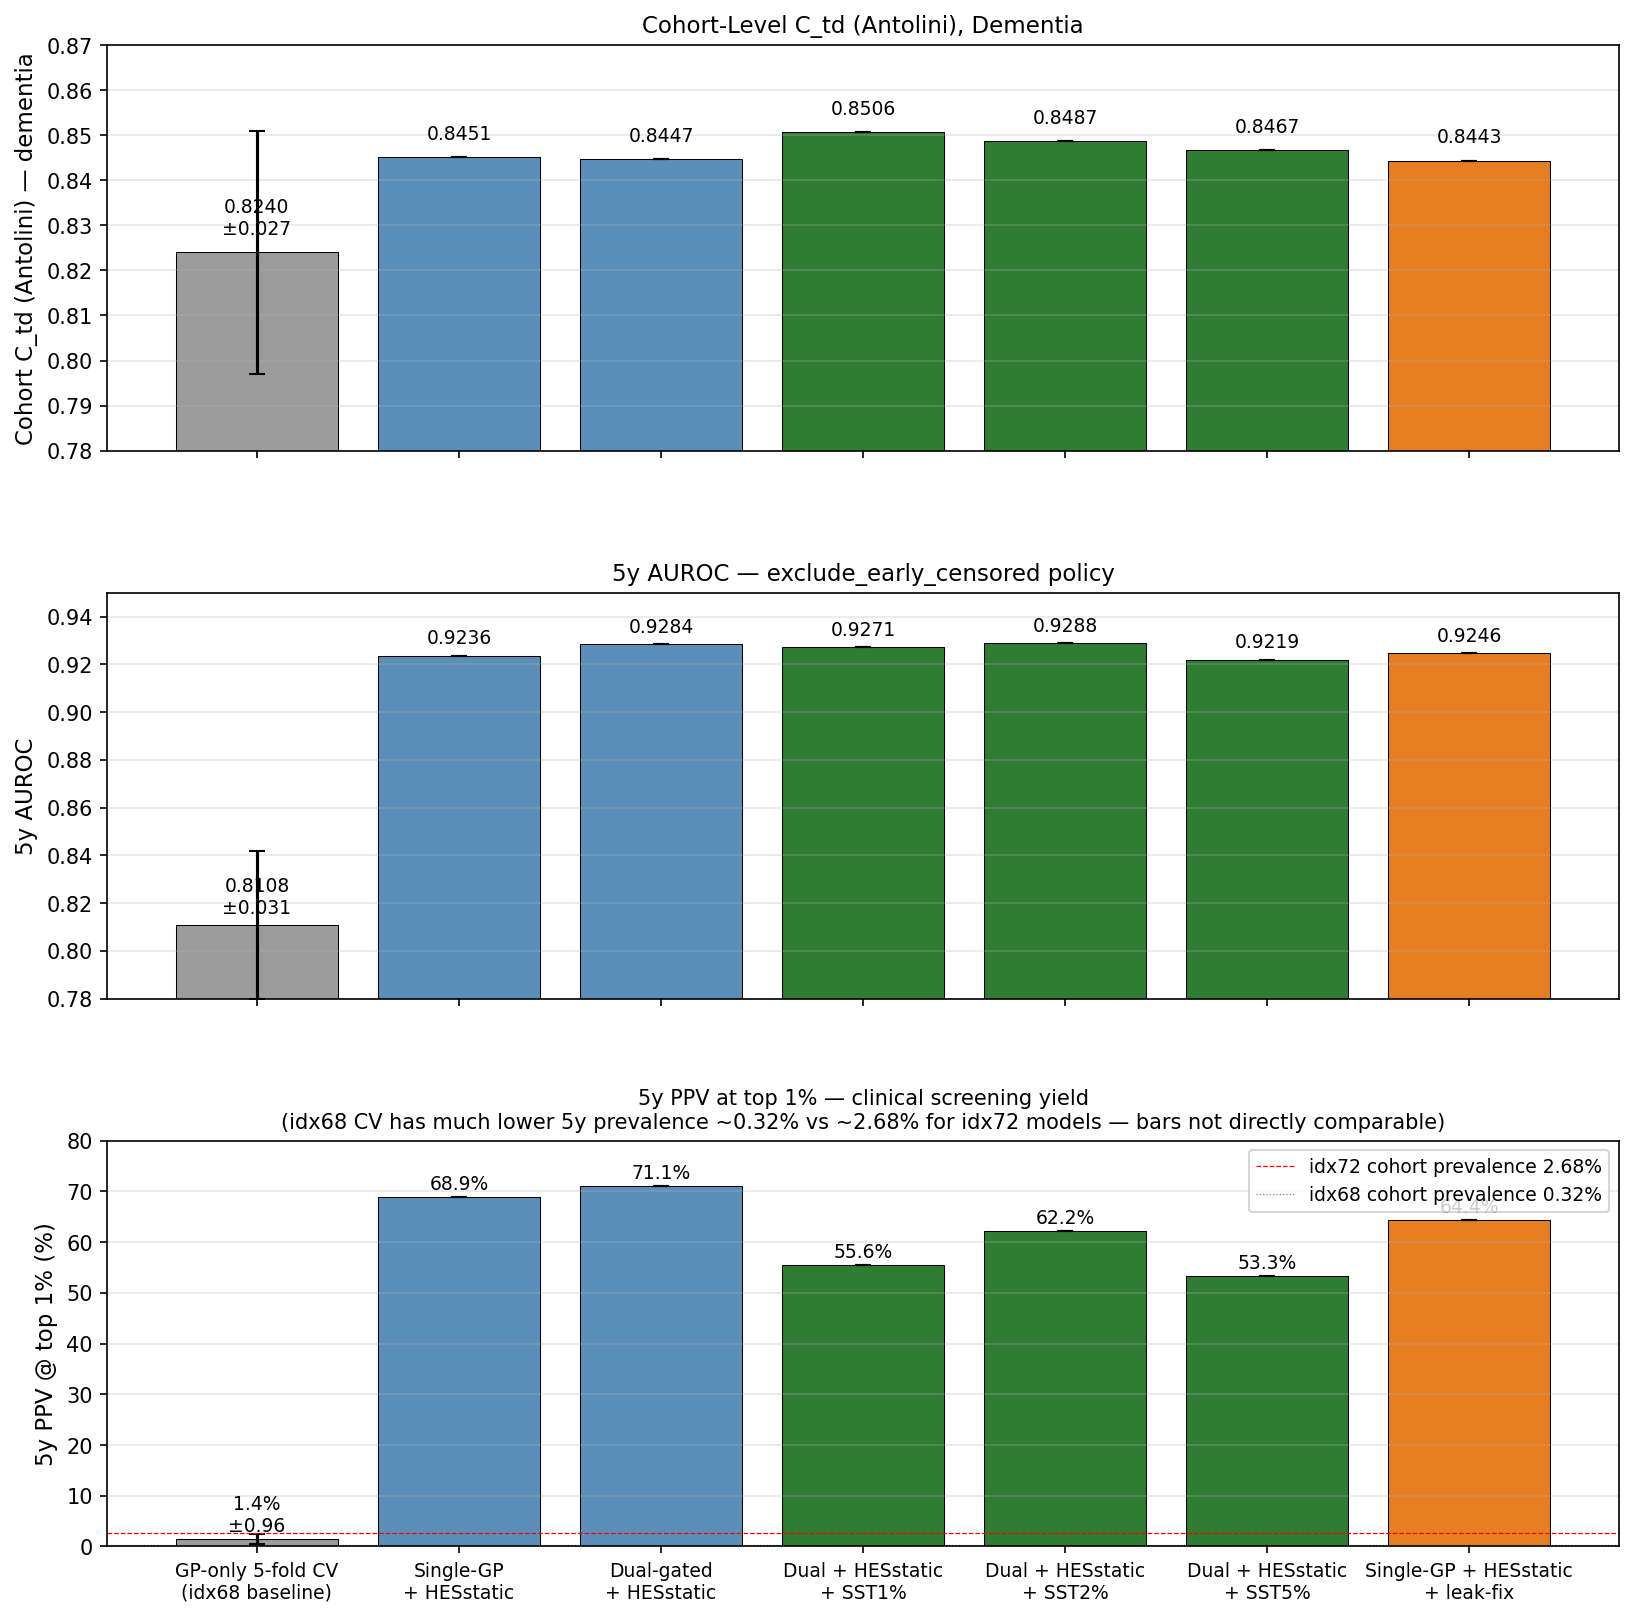
\includegraphics[keepaspectratio,alt={Model comparison}]{figs/fig_model_comparison.png}}
\caption{Model comparison}
\end{figure}

The figure shows C\_td, AUROC, and PPV@1\% across the five clean-data
models. Key observations: - \textbf{Single-GP + HESstatic ≈ Dual +
HESstatic} in C\_td and AUROC --- the dual HES backbone contributes
essentially nothing to discrimination on top of the 22-dim HES static
features. - \textbf{SST improves C\_td} at 1\% (peak), then degrades it
at 2\% and 5\%. - \textbf{PPV @ top 1\% drops with SST} ---
pseudo-labels spread the high-risk predictions wider, sacrificing
top-end precision for broader recall.

\subsubsection{7.3 SST progression}\label{sst-progression}

\begin{figure}
\centering
\pandocbounded{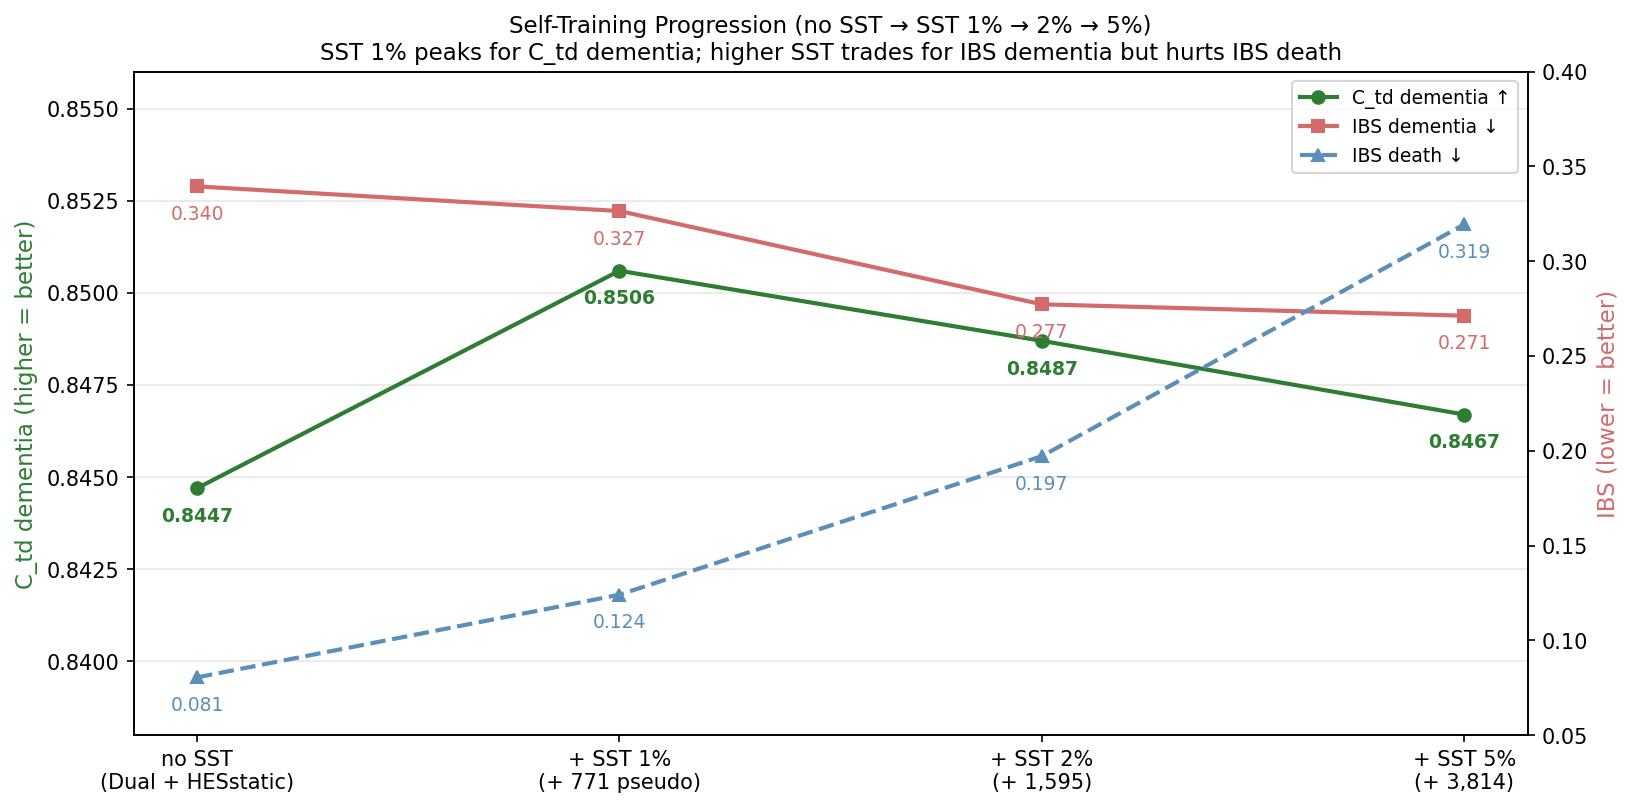
\includegraphics[keepaspectratio,alt={SST progression}]{figs/fig_sst_progression.png}}
\caption{SST progression}
\end{figure}

Going from Dual-gated + HESstatic → +SST1\% → +SST2\% → +SST5\%: -
\textbf{Dementia C\_td peaks at SST1\%} (top-1\% pseudo-labels), then
monotonically decreases as more pseudo-positives are added -
\textbf{Dementia IBS improves monotonically} (lower = better) --- more
pseudo-positives → better calibration of dementia probability -
\textbf{Death IBS degrades significantly} at SST2\% / SST5\% --- adding
many pseudo-dementia cases distorts the death-vs-dementia competing-risk
balance - → \textbf{SST1\% is the discrimination-calibration sweet spot}

\subsubsection{7.4 Where do the gains come
from?}\label{where-do-the-gains-come-from}

Decomposing the cohort-level C\_td gain along the project's
methodological journey (V2-labels-fair comparison; full per-model
numbers in Appendix B for the pre-clean models):

{\def\LTcaptype{none} % do not increment counter
\begin{longtable}[]{|>{\raggedright\arraybackslash}p{(\linewidth - 4\tabcolsep) * \real{0.3333}}|>{\raggedright\arraybackslash}p{(\linewidth - 4\tabcolsep) * \real{0.3333}}|>{\raggedright\arraybackslash}p{(\linewidth - 4\tabcolsep) * \real{0.3333}}|}
\hline
\begin{minipage}[b]{\linewidth}\raggedright
Step
\end{minipage} & \begin{minipage}[b]{\linewidth}\raggedright
From → To
\end{minipage} & \begin{minipage}[b]{\linewidth}\raggedright
ΔC\_td dementia
\end{minipage} \\
\hline
\hline
\endhead
\hline
\endlastfoot
Dual-HESaug-leak (pre-clean baseline) & --- & 0.8136 (start) \\
\hline
+ 22-dim HES static features & Dual-HESaug-leak → Dual-gated-leak &
\textbf{+0.028} ⭐ \\
\hline
+ V2 label correction (HES dementia override + DEATH cause-of-death
relabel) & Dual-gated-leak → Dual + HESstatic (clean) & +0.003 \\
\hline
+ 1st-round SST (top 1\%) & Dual + HESstatic → Dual + HESstatic + SST1\%
& +0.006 \\
\hline
\textbf{Total improvement} & & \textbf{+0.037} \\
\hline
\end{longtable}
}

\textbf{The single largest contribution is the 22-dim HES static
handcrafted features (+0.028)} --- these contribute more than any
subsequent step. Self-training and V2 label correction together add
\textasciitilde+0.009. The dual HES backbone (12M extra parameters)
contributes essentially zero on top of the 22-dim static features (see
§7.1 --- Single-GP + HESstatic and Dual-gated + HESstatic have nearly
identical C\_td).

\emph{Caveat}: The first two rows of the table (Dual-HESaug-leak and
Dual-gated-leak) were trained on V1-era data with the pre-fix HES
temporal leakage. Their cohort C\_td values (0.8136, 0.8416) are
re-evaluated against V2 labels overlaid via patient-ID match, but the
\textbf{models themselves saw leaky training data}. Consequently the
``+0.028'' gain attributed to ``+22-dim HES static'' is estimated
against a partially-leaky baseline. A clean re-test of this attribution
would require retraining Dual-HESaug on the V2 clean dataset (listed in
§10.1).

\begin{center}\rule{0.5\linewidth}{0.5pt}\end{center}

\subsection{8. Comparison with TRADE}\label{comparison-with-trade}

TRADE (NYU, Wisnivesky et al.) is the most directly comparable published
EHR foundation model for dementia prediction. It targets a broader
umbrella (AD + ADRD + MCI), uses a US EHR cohort, and reports
fixed-horizon binary metrics.

\subsubsection{8.1 Headline numbers (5-year
horizon)}\label{headline-numbers-5-year-horizon}

\begin{figure}
\centering
\pandocbounded{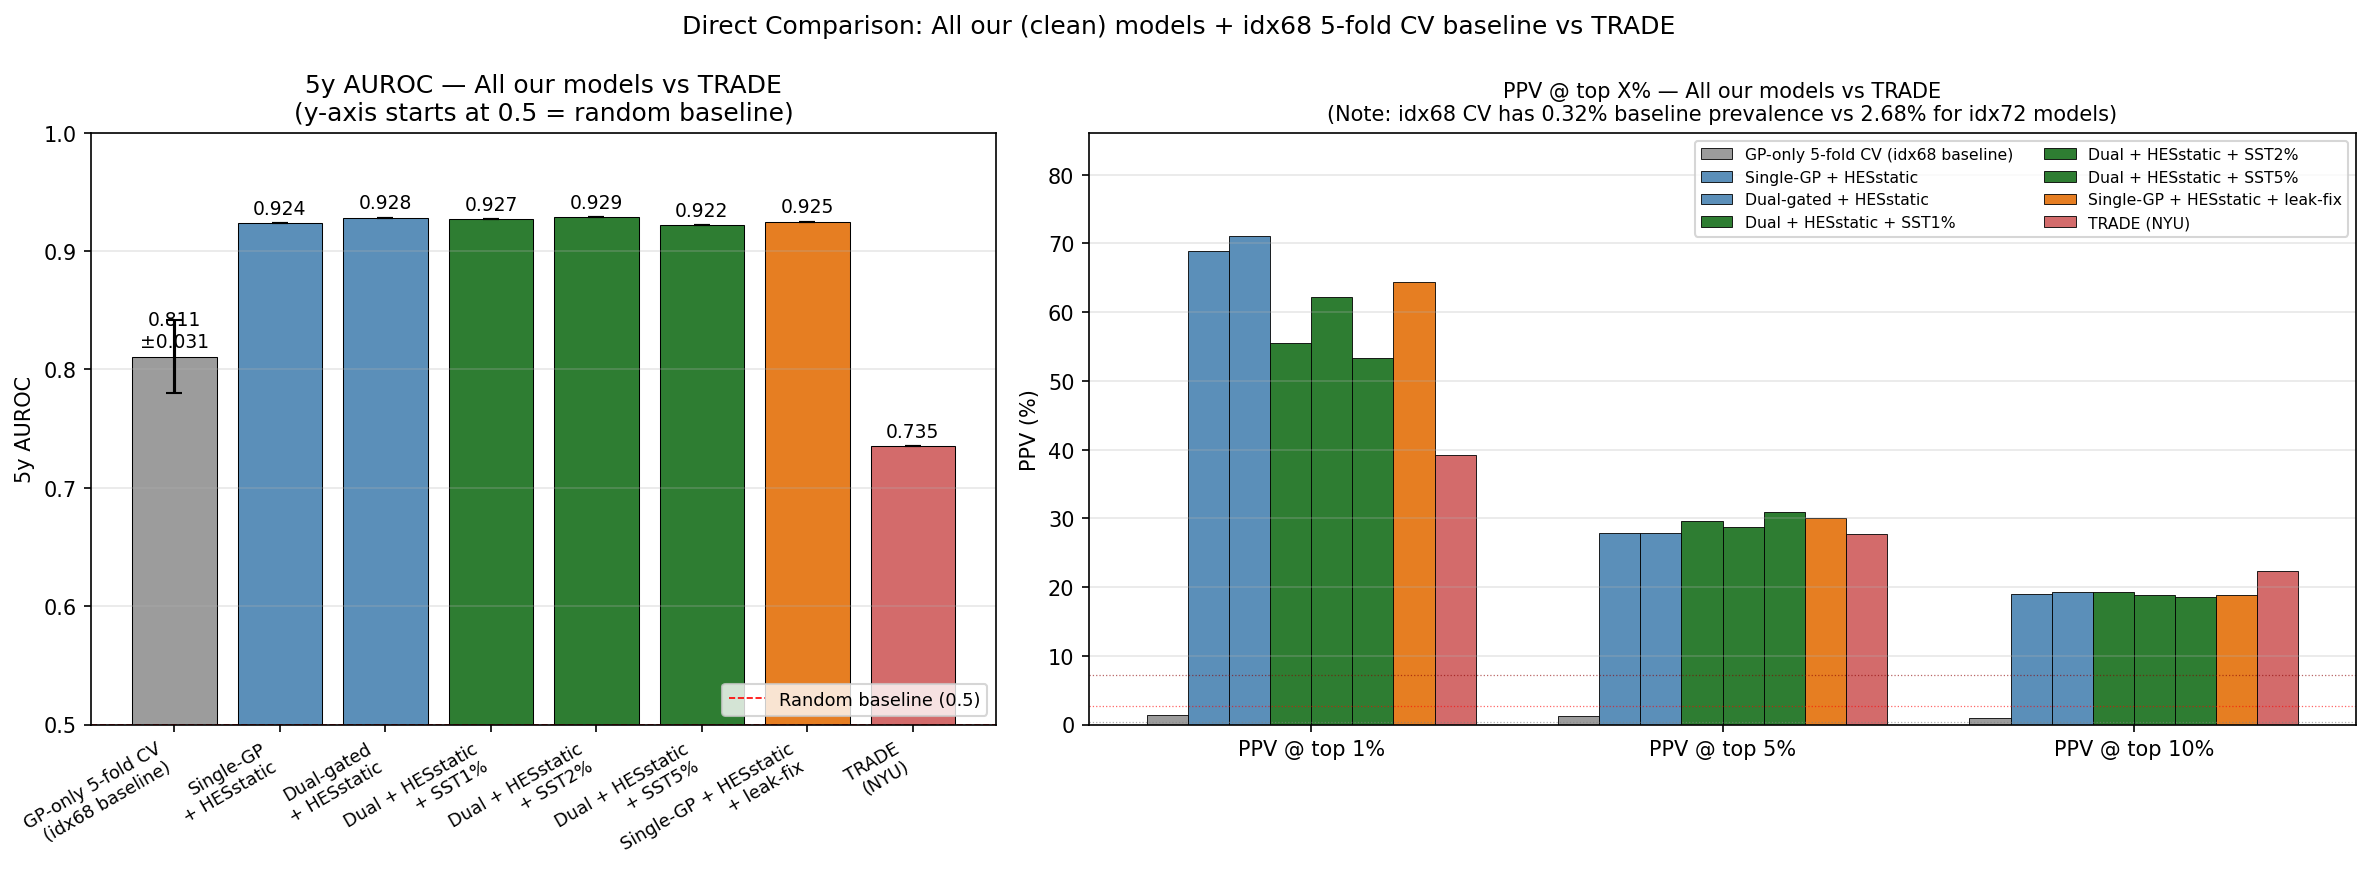
\includegraphics[keepaspectratio,alt={TRADE comparison}]{figs/fig_trade_compare.png}}
\caption{TRADE comparison}
\end{figure}

{\def\LTcaptype{none} % do not increment counter
\begin{longtable}[]{|>{\raggedright\arraybackslash}p{(\linewidth - 6\tabcolsep) * \real{0.2500}}|>{\raggedright\arraybackslash}p{(\linewidth - 6\tabcolsep) * \real{0.2500}}|>{\raggedright\arraybackslash}p{(\linewidth - 6\tabcolsep) * \real{0.2500}}|>{\raggedright\arraybackslash}p{(\linewidth - 6\tabcolsep) * \real{0.2500}}|}
\hline
\begin{minipage}[b]{\linewidth}\raggedright
Metric
\end{minipage} & \begin{minipage}[b]{\linewidth}\raggedright
TRADE
\end{minipage} & \begin{minipage}[b]{\linewidth}\raggedright
Single-GP + HESstatic (ours)
\end{minipage} & \begin{minipage}[b]{\linewidth}\raggedright
Dual + HESstatic + SST1\% (ours)
\end{minipage} \\
\hline
\hline
\endhead
\hline
\endlastfoot
5y AUROC & 0.735 & \textbf{0.9236} & \textbf{0.9271} \\
\hline
5y PPV @ top 1\% & 39.2\% & \textbf{68.89\%} & 55.56\% \\
\hline
5y PPV @ top 5\% & 27.8\% & 27.88\% & \textbf{29.65\%} \\
\hline
5y PPV @ top 10\% & 22.4\% & 19.03\% & 19.25\% \\
\hline
5y event prevalence (post-exclude-early-censored evaluable subset) &
\textasciitilde7.2\% & 121 / 4,517 = \textbf{2.68\%} & 121 / 4,517 =
\textbf{2.68\%} \\
\hline
C-index & not reported & 0.8451 & \textbf{0.8506} \\
\hline
\end{longtable}
}

\textbf{Prevalence-adjusted ``lift'' (PPV / prevalence)}:

{\def\LTcaptype{none} % do not increment counter
\begin{longtable}[]{|l|l|l|l|}
\hline
& Single-GP + HESstatic & Dual + HESstatic + SST1\% & TRADE \\
\hline
\hline
\endhead
\hline
\endlastfoot
Lift @ top 1\% & \textbf{25.7×} & 20.7× & 5.4× \\
\hline
Lift @ top 5\% & 10.4× & 11.1× & 3.9× \\
\hline
Lift @ top 10\% & 7.1× & 7.2× & 3.1× \\
\hline
\end{longtable}
}

\subsubsection{8.2 Side-by-side methodology
comparison}\label{side-by-side-methodology-comparison}

{\def\LTcaptype{none} % do not increment counter
\begin{longtable}[]{|>{\raggedright\arraybackslash}p{(\linewidth - 4\tabcolsep) * \real{0.3333}}|>{\raggedright\arraybackslash}p{(\linewidth - 4\tabcolsep) * \real{0.3333}}|>{\raggedright\arraybackslash}p{(\linewidth - 4\tabcolsep) * \real{0.3333}}|}
\hline
\begin{minipage}[b]{\linewidth}\raggedright
\end{minipage} & \begin{minipage}[b]{\linewidth}\raggedright
TRADE (NYU)
\end{minipage} & \begin{minipage}[b]{\linewidth}\raggedright
Ours
\end{minipage} \\
\hline
\hline
\endhead
\hline
\endlastfoot
Backbone & BERT-style EHR FM & SurvivEHR (GPT-style) \\
\hline
Cohort & US, NYU Langone, \textasciitilde142K patients & UK Biobank
linked GP+HES, \textasciitilde133K \\
\hline
Index policy & Sliding-window across visits (multiple samples per
patient) & Cohort entry at age 72 (one sample per patient); dynamic
prediction from latest pre-index event \\
\hline
Outcome & AD + ADRD + MCI (umbrella, \textasciitilde7.2\% 5y prevalence)
& Dementia (AD + most ADRD, no clean MCI; \textasciitilde2.68\% 5y
prevalence) \\
\hline
Output & Fixed-time binary probability & Full 25-year CIF (1,000-point
grid) for two competing causes \\
\hline
Metrics reported & AUROC, PPV@top X\% & C\_td, IBS, AUROC, PPV@top X\%,
calibration (planned) \\
\hline
Code system & ICD-10-CM (US, 5-char) & Read v2 (GP) + ICD-10 WHO (HES,
4-char) \\
\hline
\end{longtable}
}

\subsubsection{8.3 Code-set overlap
analysis}\label{code-set-overlap-analysis}

We performed an exhaustive ICD-10 code-by-code comparison between our V2
label definition and TRADE's published code list (their Table S1).

\textbf{TRADE's code list (their Table S1):}

{\def\LTcaptype{none} % do not increment counter
\begin{longtable}[]{|>{\raggedright\arraybackslash}p{(\linewidth - 2\tabcolsep) * \real{0.5000}}|>{\raggedright\arraybackslash}p{(\linewidth - 2\tabcolsep) * \real{0.5000}}|}
\hline
\begin{minipage}[b]{\linewidth}\raggedright
Bucket
\end{minipage} & \begin{minipage}[b]{\linewidth}\raggedright
ICD-10-CM codes (US)
\end{minipage} \\
\hline
\hline
\endhead
\hline
\endlastfoot
AD/ADRD & F01.\emph{, F02.}, F03.\emph{, F04.}, G23.1, G30.*, G31.01
(Pick's), G31.09 (Other FTD), G31.83 (Lewy body), G31.9 \\
\hline
MCI & G31.1, G31.84 (MCI), G31.85 (Corticobasal degen) \\
\hline
Medications & Donepezil, Galantamine, Memantine, Rivastigmine,
Tacrine \\
\hline
\end{longtable}
}

\textbf{Code-by-code comparison on UKB 133,322 cohort (HES side):}

{\def\LTcaptype{none} % do not increment counter
\begin{longtable}[]{|>{\raggedright\arraybackslash}p{(\linewidth - 6\tabcolsep) * \real{0.2500}}|>{\raggedright\arraybackslash}p{(\linewidth - 6\tabcolsep) * \real{0.2500}}|>{\raggedright\arraybackslash}p{(\linewidth - 6\tabcolsep) * \real{0.2500}}|>{\raggedright\arraybackslash}p{(\linewidth - 6\tabcolsep) * \real{0.2500}}|}
\hline
\begin{minipage}[b]{\linewidth}\raggedright
TRADE code
\end{minipage} & \begin{minipage}[b]{\linewidth}\raggedright
Patients in cohort (\%cohort)
\end{minipage} & \begin{minipage}[b]{\linewidth}\raggedright
Our HES code set
\end{minipage} & \begin{minipage}[b]{\linewidth}\raggedright
Description
\end{minipage} \\
\hline
\hline
\endhead
\hline
\endlastfoot
F01.* & 1,417 (1.06\%) & ✅ Yes & Vascular dementia \\
\hline
F02.* & 708 (0.53\%) & ✅ Yes & Dementia in other diseases (Pick's,
Parkinson's, Huntington's, CJD) \\
\hline
F03.* & 3,048 (2.29\%) & ✅ Yes & Unspecified dementia \\
\hline
F04.* & 7 (0.005\%) & ❌ No & Organic amnesic syndrome --- debatable as
dementia \\
\hline
G23.1 & 110 (0.083\%) & ❌ No & Progressive supranuclear palsy ---
movement disorder, not pure dementia \\
\hline
G30.* & 2,817 (2.11\%) & ✅ Yes & Alzheimer's disease \\
\hline
G31.0 (= US G31.01 + G31.09) & 119 (0.089\%) & ❌ \textbf{MISSED} &
Pick's disease / circumscribed brain atrophy --- should be added \\
\hline
G31.8 (= US G31.83 + G31.85 + Lewy body etc.) & 530 (0.398\%) & ❌
\textbf{MISSED} & Other degenerative --- includes Lewy body dementia \\
\hline
G31.9 & 1,173 (0.880\%) & ❌ No & Unspecified neurodegen --- debatable
as dementia \\
\hline
G31.1 & 17 (0.013\%) & ❌ No & Senile degen NEC (TRADE's MCI bucket) \\
\hline
\textbf{G31.84 (MCI)} & \textbf{0} & ❌ N/A & \textbf{Does not exist in
WHO ICD-10 --- UK has no equivalent} \\
\hline
G31.85 (Corticobasal) & folds into G31.8 (530) & ❌ partial & Falls
under G31.8 in WHO \\
\hline
Dementia meds & not included & ❌ No & We do not use medication-based
label triggers \\
\hline
\end{longtable}
}

Note: WHO ICD-10 (used in UK HES) has only 4-character resolution. The
US ICD-10-CM 5-character extensions G31.83 (Lewy body) and G31.84 (MCI)
are not representable. The closest mapping is
\passthrough{\lstinline!G31.0 → US G31.01/.09!} and
\passthrough{\lstinline!G31.8 → US G31.83/.85!}.

\subsubsection{8.4 Set overlap
visualisation}\label{set-overlap-visualisation}

\begin{figure}
\centering
\pandocbounded{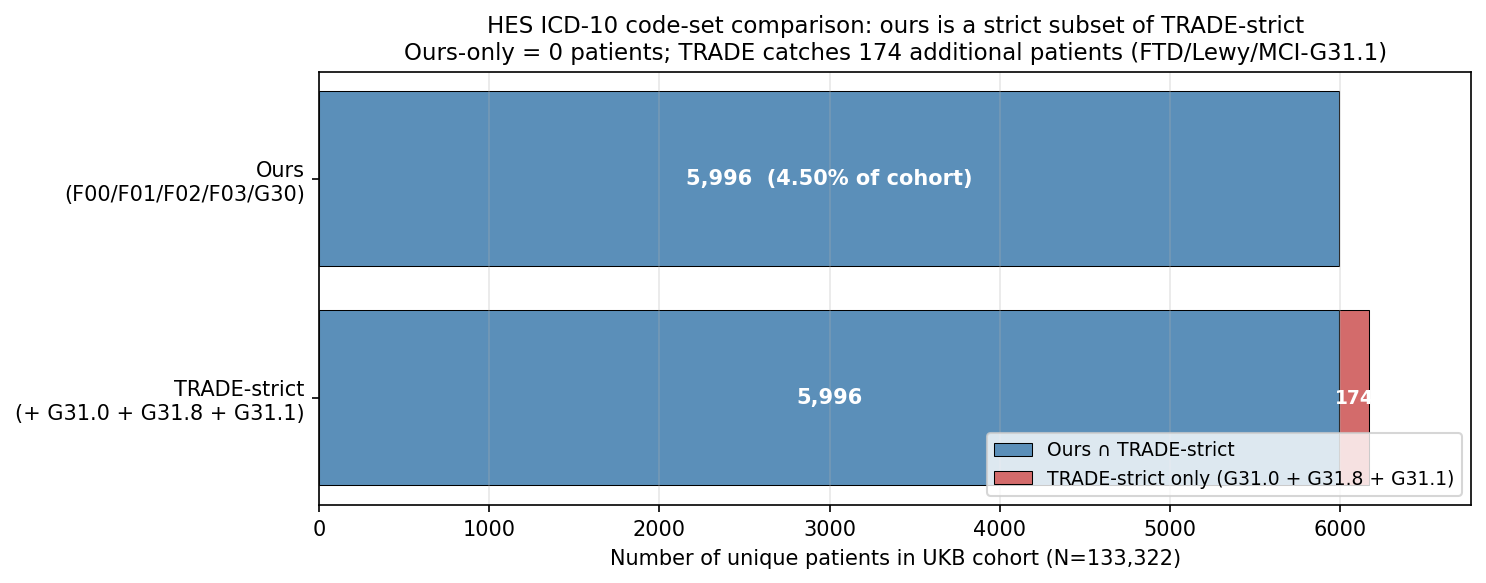
\includegraphics[keepaspectratio,alt={Code overlap stacked bar}]{figs/fig_code_overlap.png}}
\caption{Code overlap stacked bar}
\end{figure}

\textbf{Quantitative summary (133K UKB cohort, HES side)}:

{\def\LTcaptype{none} % do not increment counter
\begin{longtable}[]{|>{\raggedright\arraybackslash}p{(\linewidth - 4\tabcolsep) * \real{0.3333}}|>{\raggedright\arraybackslash}p{(\linewidth - 4\tabcolsep) * \real{0.3333}}|>{\raggedright\arraybackslash}p{(\linewidth - 4\tabcolsep) * \real{0.3333}}|}
\hline
\begin{minipage}[b]{\linewidth}\raggedright
Set
\end{minipage} & \begin{minipage}[b]{\linewidth}\raggedright
Patients
\end{minipage} & \begin{minipage}[b]{\linewidth}\raggedright
\%cohort
\end{minipage} \\
\hline
\hline
\endhead
\hline
\endlastfoot
Ours (F00 ∪ F01 ∪ F02 ∪ F03 ∪ G30) & 5,996 & 4.50\% \\
\hline
TRADE-strict (adds G31.0, G31.8, G31.1 --- clean dementia subtypes) &
6,170 & 4.63\% \\
\hline
TRADE-full (adds also G31.9, F04, G23.1 --- debatable) & 7,026 &
5.27\% \\
\hline
\textbf{Intersection: ours ∩ TRADE} & \textbf{5,996} & (100\% of
ours) \\
\hline
Only in ours (not in TRADE) & 0 & --- \\
\hline
Only in TRADE-strict (not in ours) & 174 & 0.13\% \\
\hline
Only in TRADE-full & 1,030 & 0.77\% \\
\hline
\end{longtable}
}

\textbf{Interpretation}: - Our HES dementia set is a \textbf{strict
subset} of TRADE's umbrella (100\% of our patients are in TRADE). -
TRADE catches \textbf{174 additional patients} (vs ours, strict
comparison) --- mostly Lewy body (G31.8, 148 unique) and Pick's/FTD
(G31.0, 13 unique). - The ``debatable'' TRADE addition (G31.9
unspecified neurodegen) accounts for 1,030 of the 1,030 extras under the
full umbrella --- 88\% of the gap is from a single code that may not
represent dementia per se. - \textbf{MCI is fundamentally
unrepresentable in UK ICD-10}. The 22 patients labeled
\passthrough{\lstinline!Eu057!} (the closest available Read code,
mapping to F06.7 ``Mild cognitive disorder due to brain damage'') is a
different clinical construct than Petersen MCI.

\subsubsection{8.5 If we extended our
label}\label{if-we-extended-our-label}

To match TRADE more closely we could: - \textbf{Add G31.0 + G31.8 (clean
dementia subtypes)} → +161 patients in cohort (+2.7\% relative) → new
label N=6,157 (4.62\% of cohort) --- essentially matching TRADE-strict
(4.63\%). Easy fix, would require re-running V2 dataset build. -
\textbf{Add G31.9} → +1,030 patients but introduces non-dementia noise.
Not recommended. - \textbf{Add dementia medications} (Donepezil etc.,
BNF-coded in GP) → could meaningfully expand to MCI-like patients on
memory medications. Would require new code list curation and dataset
rebuild.

\subsubsection{8.6 AUROC / PPV computation
verification}\label{auroc-ppv-computation-verification}

The AUROC and PPV numbers in this report were independently verified by
three computations: 1. sklearn \passthrough{\lstinline!roc\_auc\_score!}
2. Manual Mann-Whitney U statistic via numpy ranks 3. Direct all-pairs
enumeration (every positive--negative pair compared explicitly)

All three methods agree to 1e-16 on Dual + HESstatic + SST1\%'s 5y AUROC
of 0.9271. The cohort-level computation has no batching, no
order-dependence, no censoring-weighting model --- methodology issues
like the per-batch C\_td bug (see Appendix A) cannot recur here.

\begin{center}\rule{0.5\linewidth}{0.5pt}\end{center}

\subsection{9. Where Our Work Sits in the
Literature}\label{where-our-work-sits-in-the-literature}

Brief context --- these are not direct apples-to-apples comparisons
because of cohort/task differences:

{\def\LTcaptype{none} % do not increment counter
\begin{longtable}[]{|>{\raggedright\arraybackslash}p{(\linewidth - 8\tabcolsep) * \real{0.2000}}|>{\raggedright\arraybackslash}p{(\linewidth - 8\tabcolsep) * \real{0.2000}}|>{\raggedright\arraybackslash}p{(\linewidth - 8\tabcolsep) * \real{0.2000}}|>{\raggedright\arraybackslash}p{(\linewidth - 8\tabcolsep) * \real{0.2000}}|>{\raggedright\arraybackslash}p{(\linewidth - 8\tabcolsep) * \real{0.2000}}|}
\hline
\begin{minipage}[b]{\linewidth}\raggedright
Paper
\end{minipage} & \begin{minipage}[b]{\linewidth}\raggedright
Cohort
\end{minipage} & \begin{minipage}[b]{\linewidth}\raggedright
Task
\end{minipage} & \begin{minipage}[b]{\linewidth}\raggedright
Approach
\end{minipage} & \begin{minipage}[b]{\linewidth}\raggedright
Reported 5y AUROC
\end{minipage} \\
\hline
\hline
\endhead
\hline
\endlastfoot
\textbf{SurvivEHR} (Gadd 2025) & 23M CPRD pretraining → various FFT
tasks & 19 multi-long-term conditions & Same backbone we use & 0.79 for
dementia (different prediction setup) \\
\hline
\textbf{TRADE} (Wisnivesky NYU, undated) & 142K NYU Langone EHR &
AD/ADRD/MCI binary & BERT-style EHR FM & 0.735 \\
\hline
\textbf{eRADAR} (NYU baseline) & (same as TRADE) & AD/ADRD/MCI &
Logistic regression (hand features) & 0.688 \\
\hline
\textbf{PROMISE-AD} (Lyu et al.~2026, Yale) & ADNI/TADPOLE,
\textasciitilde1.7K & CN→MCI, MCI→AD conversion & Tabular transformer +
survival & 0.84 (CN→MCI), 0.997 (MCI→AD) --- different paradigm \\
\hline
\textbf{DemRisk} (Reeves 2024) & UK CPRD GOLD, \textasciitilde400K & 5y
dementia & Cox proportional hazards & 0.78 \\
\hline
\textbf{Ours (Single-GP + HESstatic)} & 133K UKB GP+HES & Dementia 25y
CIF & SurvivEHR + 22-dim HES static & 0.9236 \\
\hline
\textbf{Ours (Dual + HESstatic + SST1\%)} & 133K UKB GP+HES & Dementia
25y CIF & + dual backbone + 1\% SST & 0.9271 \\
\hline
\end{longtable}
}

TRADE is the only directly comparable foundation-model EHR work on a
dementia umbrella; PROMISE-AD operates in a completely different
paradigm (MCI→AD biomarker-driven, ADNI cohort). The numerical gap to
TRADE is large (\textasciitilde+0.19 AUROC) but the cohort and task
differences are equally large --- the \textbf{methodological message is
that competing-risk modeling + dynamic prediction + foundation-model
backbone yields strong discrimination on UK primary-care data}.

\begin{center}\rule{0.5\linewidth}{0.5pt}\end{center}

\subsection{10. Open Questions and Next
Steps}\label{open-questions-and-next-steps}

\subsubsection{10.1 Re-run prior experiments on clean data + complete
the leak-fixed SST round + idx72 GP-only
CV}\label{re-run-prior-experiments-on-clean-data-complete-the-leak-fixed-sst-round-idx72-gp-only-cv}

\begin{enumerate}
\def\labelenumi{\arabic{enumi}.}
\tightlist
\item
  \textbf{GP-only 5-fold CV at idx age 72} \emph{(in progress)} ---
  replacement for the current idx68 row in §7.1, on the matching cohort.
  Each of 5 folds will be trained with single GP backbone, no HES at
  all, idx age 72, V2 clean labels. Will be the cleanest non-HES
  baseline.
\item
  \textbf{Run the SST1\% round on top of the leakage-fixed base model}
  --- the base is already trained and tested (Single-GP + HESstatic +
  leak-fix in §7.1: C\_td dem 0.8443, AUROC 0.9246, IBS dem 0.2887).
  Next step: run inference on the leakage-cleaned training set, select
  top-1\% censored as pseudo-positives with empirical-lag-sampled event
  times, retrain. Expected to slightly improve PPV@5\% and IBS dem
  (matches V2-Dual → SST1\% trajectory).
\item
  \textbf{Retrain the dual-cross-attention model on V2 clean dataset}
  --- not yet done; would isolate whether cross-attention vs gated
  fusion matters on clean data. The pre-leakage comparison
  (Dual-XAttn-leak ≈ Dual-gated-leak within 0.001) suggests no, but
  should be verified.
\item
  \textbf{Retrain Dual-HESaug on V2 clean dataset} --- could match or
  surpass Single-GP + HESstatic since HESaug used a slightly different
  label augmentation strategy.
\item
  \textbf{Retrain GP+HESseq-fusion on V2 clean dataset} --- even if it
  still fails on clean data, the negative result is publishable evidence
  that sequence fusion of two long EHR token streams is not the right
  strategy.
\end{enumerate}

\subsubsection{10.2 Extend the dementia code
definition}\label{extend-the-dementia-code-definition}

Current label is 41 Read v2 codes + 5 HES ICD-10 families. Multiple
extensions worth piloting:

{\def\LTcaptype{none} % do not increment counter
\begin{longtable}[]{|>{\raggedright\arraybackslash}p{(\linewidth - 6\tabcolsep) * \real{0.2500}}|>{\raggedright\arraybackslash}p{(\linewidth - 6\tabcolsep) * \real{0.2500}}|>{\raggedright\arraybackslash}p{(\linewidth - 6\tabcolsep) * \real{0.2500}}|>{\raggedright\arraybackslash}p{(\linewidth - 6\tabcolsep) * \real{0.2500}}|}
\hline
\begin{minipage}[b]{\linewidth}\raggedright
Extension
\end{minipage} & \begin{minipage}[b]{\linewidth}\raggedright
Expected new patients in cohort
\end{minipage} & \begin{minipage}[b]{\linewidth}\raggedright
Effort
\end{minipage} & \begin{minipage}[b]{\linewidth}\raggedright
Rationale
\end{minipage} \\
\hline
\hline
\endhead
\hline
\endlastfoot
Add \passthrough{\lstinline!G31.0!} + \passthrough{\lstinline!G31.8!} to
HES list & +161 (+2.7\%) & Low (rebuild dataset) & Clean dementia
subtypes (Pick's/FTD + Lewy body) currently missed \\
\hline
Add dementia medications (BNF: Donepezil, Galantamine, Memantine,
Rivastigmine, Tacrine) & likely +500-1500 & Medium (need BNF code
curation) & Many MCI / early-dementia patients are on memory medications
without a formal dementia code. Matches TRADE's strategy. \\
\hline
Add UK MCI-proxy Read codes (\passthrough{\lstinline!1B1F.!} memory
loss, \passthrough{\lstinline!E260.!} cognitive impairment,
\passthrough{\lstinline!1S4..!} etc.) & likely +200-800 & Medium
(clinical curation) & Closes the MCI gap with TRADE (G31.84 has no WHO
equivalent) \\
\hline
Add \passthrough{\lstinline!G31.9!} (degenerative NS unspecified) &
+1,030 (\textasciitilde17\% relative gain) & Trivial & TRADE includes;
debatable as pure dementia \\
\hline
\end{longtable}
}

The medication-based and MCI-Read-code extensions should be discussed
with a clinical collaborator before adoption.

\subsubsection{10.3 Extend the HES static covariate
vector}\label{extend-the-hes-static-covariate-vector}

Current 22-dim HES static is mostly cardiovascular + a few neurological
/ metabolic flags. Reasonable extensions:

{\def\LTcaptype{none} % do not increment counter
\begin{longtable}[]{|>{\raggedright\arraybackslash}p{(\linewidth - 4\tabcolsep) * \real{0.3333}}|>{\raggedright\arraybackslash}p{(\linewidth - 4\tabcolsep) * \real{0.3333}}|>{\raggedright\arraybackslash}p{(\linewidth - 4\tabcolsep) * \real{0.3333}}|}
\hline
\begin{minipage}[b]{\linewidth}\raggedright
Extension
\end{minipage} & \begin{minipage}[b]{\linewidth}\raggedright
Dimensions
\end{minipage} & \begin{minipage}[b]{\linewidth}\raggedright
Rationale
\end{minipage} \\
\hline
\hline
\endhead
\hline
\endlastfoot
Add finer-grained ICD-10 chapters & +20-30 dims & Currently we don't
have flags for many neurodegenerative-adjacent conditions (e.g., sleep
apnea, head injury subtypes, mood disorders by severity, anxiety
disorders by type) \\
\hline
Add medication-class summaries (BNF chapter level) & +30-50 dims &
Medication burden, statin use, anticholinergic load, antidepressant use
--- all associated with dementia risk \\
\hline
Add lab-test summary statistics (HbA1c trajectory slope, blood pressure
trajectory, eGFR slope) & +10-20 dims & Cardiovascular / metabolic risk
trajectories are robust dementia predictors \\
\hline
Add social / lifestyle aggregates from GP & +5-10 dims & Smoking ever /
pack-years, alcohol intake bands, BMI trajectory \\
\hline
\end{longtable}
}

Target: \textbf{\textasciitilde100-150 dim HES static vector} vs current
22.

\subsubsection{10.4 Use more data}\label{use-more-data}

The current model uses \textasciitilde133K UKB patients with idx age 72.
Several expansion paths:

\begin{enumerate}
\def\labelenumi{\arabic{enumi}.}
\tightlist
\item
  \textbf{Drop the fixed idx-age constraint} --- train on all UKB-linked
  GP patients with sufficient diagnostic history. The 230K figure quoted
  earlier (§2.3) is the count of UKB participants with ≥1 diagnostic
  record in \passthrough{\lstinline!diagnosis\_table!}; the full GP
  linkage \passthrough{\lstinline!static\_table!} is 502K. Removing the
  idx-age 72 constraint would let us include patients with index points
  other than age 72 (subject to ≥5 events / ≥1y registration etc.),
  potentially several-fold more than our current 133K. Requires
  re-thinking the prediction setup (sliding-window or random-index
  instead of fixed age 72).
\item
  \textbf{Use the full SurvivEHR pretraining pool} (23M CPRD-linked GP
  patients) for further pretraining on a broader cohort, then fine-tune
  on the UKB subset. SurvivEHR's reported pretraining already uses this.
\item
  \textbf{Multi-source fine-tuning}: combine UKB with CPRD GOLD or other
  UK primary-care datasets if available.
\end{enumerate}

\subsubsection{10.5 Add APOE genotype}\label{add-apoe-genotype}

UK Biobank has genome-wide genotyping (\textasciitilde488K
participants). \textbf{APOE ε4 allele count is the strongest single
genetic risk factor for late-onset Alzheimer's disease} --- homozygous
ε4/ε4 carriers have \textasciitilde15× lifetime risk vs ε3/ε3.

Implementation: - Extract APOE ε2 / ε3 / ε4 dosage from UKB genotype
data - Add as a 3-dim feature (or compact one-hot of 6 genotype
combinations) - Expected effect: significant lift on top-percentile PPV,
particularly at older ages

This is the single most clinically motivated covariate addition.

\subsubsection{10.6 Add UmlsBERT-style domain knowledge
augmentation}\label{add-umlsbert-style-domain-knowledge-augmentation}

\textbf{Motivation}: Our backbone learned representations purely from
co-occurrence in EHR sequences. It does not know that
\passthrough{\lstinline!J16y4!} (stomach disorder) and
\passthrough{\lstinline!J51..!} (diaphragm disorder) are both
``digestive system pathologies'', or that
\passthrough{\lstinline!Eu023!} and \passthrough{\lstinline!G20..!} are
both linked to Parkinson's disease. UmlsBERT (Michalopoulos et al.,
2021, NAACL) showed that injecting UMLS Metathesaurus structure into a
clinical language model improves downstream NER and NLI tasks.

\begin{quote}
``UmlsBERT integrates domain knowledge during pre-training via two
strategies: (i) connecting words that have the same underlying `concept'
in UMLS, and (ii) leveraging semantic type knowledge in UMLS to create
clinically meaningful input embeddings.''
\end{quote}

Two integration paths for our SurvivEHR backbone:

\begin{enumerate}
\def\labelenumi{\arabic{enumi}.}
\tightlist
\item
  \textbf{Token-level concept embedding} --- for each Read v2 / ICD-10
  code in our vocabulary, look up its UMLS CUI (concept unique
  identifier) and semantic type. Add a learned embedding for the CUI
  and/or semantic type to each token's input embedding. This injects
  structured ``what kind of clinical thing is this'' knowledge.
\item
  \textbf{Knowledge-augmented continued pretraining} --- continue
  pretraining the SurvivEHR backbone with an auxiliary objective that
  pulls codes with the same UMLS concept closer in embedding space.
  Could use a MASK-then-predict-CUI task analogous to UmlsBERT's masked
  LM with concept distribution.
\end{enumerate}

Expected benefits: - Better few-shot generalization to rare codes (most
of our 41 dementia codes have \textless10 patients) - Better
cross-vocabulary alignment between Read v2 (GP) and ICD-10 (HES) ---
currently the model has to learn this from co-occurrence statistics -
Improved interpretability --- embeddings would cluster by semantic type

Implementation cost is moderate (UMLS license is free for research; CUI
lookup is straightforward via QuickUMLS or RxNorm).

\subsubsection{10.7 Methodological
improvements}\label{methodological-improvements}

\begin{enumerate}
\def\labelenumi{\arabic{enumi}.}
\tightlist
\item
  \textbf{IPCW-AUC} (Inverse Probability of Censoring Weighting) as a
  principled alternative to the ``exclude early-censored'' policy ---
  most rigorous censoring-aware AUC estimator. Recommended as the
  headline metric for the final paper.
\item
  \textbf{Report time-dependent AUC} at horizons 1, 2, 3, 5, 10y to show
  how discrimination changes with horizon.
\item
  \textbf{External validation cohort} --- currently all evaluation is
  in-sample on UKB. A held-out cohort like CPRD GOLD or US Optum would
  strengthen the paper substantially.
\end{enumerate}

\begin{center}\rule{0.5\linewidth}{0.5pt}\end{center}

\subsection{Appendix A: Methodology corrections (project
history)}\label{appendix-a-methodology-corrections-project-history}

These corrections are not central to the headline narrative but were
important learnings.

\subsubsection{A.1 Per-batch C\_td averaging
artifact}\label{a.1-per-batch-c_td-averaging-artifact}

The default Lightning training callback aggregates C\_td \textbf{per
batch} then averages across batches. This is not a bug in the strict
sense --- it's the callback's default aggregation --- but it produces
values that are not equivalent to cohort-level C\_td. With batch size
16: - 47\% of batches contained 0 dementia events, making per-batch
C\_td numerically unstable. - Cross-batch (positive, negative) ranking
pairs were lost. - Result was order-dependent: sequential vs shuffled
batching changed mean C\_td by +0.078. - Reported C\_td values were
systematically \textbf{understated by \textasciitilde0.07-0.10 absolute}
(e.g., Dual + HESstatic + SST1\% per-batch = 0.7685 vs cohort-level =
0.8506).

\textbf{Fix}: Compute C\_td at the cohort level using
\passthrough{\lstinline!pycox.EvalSurv.concordance\_td('antolini')!} on
the full test set in a single pass (script:
\passthrough{\lstinline!compute\_cohort\_ctd\_generic.py!}; see
\passthrough{\lstinline!COHORT\_CTD\_RESULTS.md!} for the authoritative
numbers used in §7.1). Cross-verified with a manual numpy implementation
(Wolbers 2014 competing-risk extension); cause-specific and
true-competing-risk C\_td differ by \textless0.005 on our data. All
numbers in §7 are cohort-level from this script.

\subsubsection{A.2 GP-prevalent label
leakage}\label{a.2-gp-prevalent-label-leakage}

In the V1 dataset, \textbf{246 test/train/val patients had a GP dementia
code recorded before their cohort entry date} (idx age 72) but were
still included as candidates for the dementia event. This is a temporal
leakage: they were prevalent cases, not incident cases.

\textbf{Fix}: The latest ``Single-GP + HESstatic + leak-fix'' model uses
a rebuilt base dataset that removes these 246 patients (213 train / 17
val / 16 test). Test-set numbers in §7 already exclude the 16 test-set
leaky patients (canonical 8,241 cohort).

\subsubsection{A.3 25-year horizon
clarification}\label{a.3-25-year-horizon-clarification}

We initially believed the model predicted a 5-year horizon. After
investigating the empirical pseudo-event lag distribution (median 8.8y,
max 16y for true V1-Type-C alive-censored patients), we discovered the
actual model horizon is 25 years:
\passthrough{\lstinline!time\_scale = 1825 days × supervised\_time\_scale = 5 = 9,125 days ≈ 25 years!}.
The normalised \passthrough{\lstinline!t\_eval ∈ [0, 1]!} therefore maps
to \passthrough{\lstinline![0, 25 years]!}. All metrics in §7 are
computed against this correct horizon, with
\passthrough{\lstinline!t\_eval[200] = 0.2002 ≈ 5.005y!} used for ``5y''
results.

\subsubsection{A.4 Pre-leakage era HES temporal
filtering}\label{a.4-pre-leakage-era-hes-temporal-filtering}

In V1 datasets, HES records were not strictly filtered to
\passthrough{\lstinline!admidate < index\_date!}. This meant patients
whose dementia diagnosis was recorded in HES after age 72 could still
have features influenced by post-index admissions --- a form of temporal
data leakage.

\textbf{Fix}: The V2 clean dataset rebuilds the 22-dim HES static
feature vector with strict pre-index filtering
(\passthrough{\lstinline!admidate < index\_date!}, plus dementia codes
excluded). V2 clean labels also use cleaner cause-of-death coding. The
pre-leakage experiments (Dual-HESaug, GP+HESseq-fusion, Dual-gated,
Dual-XAttn) were trained before this fix. The GP-only 5-fold CV baseline
(idx age 68) does not have HES temporal leakage (uses no HES data) but
is on a different cohort --- see §7.1.

\begin{center}\rule{0.5\linewidth}{0.5pt}\end{center}

\subsection{Appendix B: Pre-clean (leakage-era)
experiments}\label{appendix-b-pre-clean-leakage-era-experiments}

The following experiments were trained on the V1 dataset, where
pre-index HES dementia codes were not always strictly excluded from the
static feature vector (temporal leakage), and labels did not include the
V2 corrections. We re-evaluated them at the cohort level with V2 labels
overlaid via patient-ID match to enable fair comparison; their numbers
should not be treated as headline results.

{\def\LTcaptype{none} % do not increment counter
\begin{longtable}[]{|>{\raggedright\arraybackslash}p{(\linewidth - 2\tabcolsep) * \real{0.5000}}|>{\raggedright\arraybackslash}p{(\linewidth - 2\tabcolsep) * \real{0.5000}}|}
\hline
\begin{minipage}[b]{\linewidth}\raggedright
Short name
\end{minipage} & \begin{minipage}[b]{\linewidth}\raggedright
Architecture
\end{minipage} \\
\hline
\hline
\endhead
\hline
\endlastfoot
\textbf{Dual-HESaug-leak} & Single GP backbone + HES label augmentation
+ 22-dim HES static \\
\hline
\textbf{GP+HESseq-fusion-leak} & Single backbone with HES events fused
INTO the GP token sequence (failed approach --- sequence becomes too
long and 60\% gets truncated) \\
\hline
\textbf{Dual-gated-leak} & Dual GP+HES backbones, gated fusion, + 22-dim
HES static \\
\hline
\textbf{Dual-XAttn-leak} & Dual GP+HES backbones, cross-attention
fusion, + 22-dim HES static \\
\hline
\end{longtable}
}

Cohort-level C\_td (dementia) on V2 canonical 8,241 test cohort, V2
labels overlaid:

{\def\LTcaptype{none} % do not increment counter
\begin{longtable}[]{|>{\raggedright\arraybackslash}p{(\linewidth - 6\tabcolsep) * \real{0.2500}}|>{\raggedright\arraybackslash}p{(\linewidth - 6\tabcolsep) * \real{0.2500}}|>{\raggedright\arraybackslash}p{(\linewidth - 6\tabcolsep) * \real{0.2500}}|>{\raggedright\arraybackslash}p{(\linewidth - 6\tabcolsep) * \real{0.2500}}|}
\hline
\begin{minipage}[b]{\linewidth}\raggedright
Model
\end{minipage} & \begin{minipage}[b]{\linewidth}\raggedright
Cohort tested on
\end{minipage} & \begin{minipage}[b]{\linewidth}\raggedright
Cohort C\_td dem
\end{minipage} & \begin{minipage}[b]{\linewidth}\raggedright
Note
\end{minipage} \\
\hline
\hline
\endhead
\hline
\endlastfoot
Dual-HESaug-leak & V2 canonical 8,241 (V2 labels overlay) &
\textbf{0.8136} & fair vs clean models \\
\hline
GP+HESseq-fusion-leak & V2 canonical 8,241 & \textbf{0.7098} &
sequence-fusion approach fails: −0.10 vs Dual-HESaug-leak \\
\hline
Dual-gated-leak & V2 canonical (V2 labels) & \textbf{0.8416} & dual
backbone trained on V1 labels \\
\hline
Dual-XAttn-leak & V2 canonical (V2 labels) & \textbf{0.8428} &
cross-attn ≈ gated \\
\hline
\end{longtable}
}

Key methodological lessons from these pre-clean experiments: -
\textbf{Sequence fusion of GP + HES into one token stream fails} --- the
combined sequence median is \textasciitilde731 tokens vs the model's
block size 512, so 60\% of patients get truncated. Late fusion (dual
backbone or static features) is strictly better. - \textbf{Gated fusion
≈ cross-attention} within 0.001 C\_td --- the fusion mechanism is not
where the gains live. - \textbf{Dual backbone ≈ single backbone + 22-dim
HES static} within 0.001 --- the dual model's second backbone is
essentially redundant once the 22-dim static features are present (later
verified on clean V2 data).

\begin{center}\rule{0.5\linewidth}{0.5pt}\end{center}

\subsection{Appendix C: Key files}\label{appendix-c-key-files}

{\def\LTcaptype{none} % do not increment counter
\begin{longtable}[]{|>{\raggedright\arraybackslash}p{(\linewidth - 2\tabcolsep) * \real{0.5000}}|>{\raggedright\arraybackslash}p{(\linewidth - 2\tabcolsep) * \real{0.5000}}|}
\hline
\begin{minipage}[b]{\linewidth}\raggedright
Item
\end{minipage} & \begin{minipage}[b]{\linewidth}\raggedright
Path
\end{minipage} \\
\hline
\hline
\endhead
\hline
\endlastfoot
Project plan & \passthrough{\lstinline!CPRD/PROJECT\_KNOWLEDGE.md!} \\
\hline
Cohort C\_td results (all models) &
\passthrough{\lstinline!CPRD/COHORT\_CTD\_RESULTS.md!} \\
\hline
Methodology audit &
\passthrough{\lstinline!CPRD/CTD\_CORRECTION\_AUDIT\_2026-05-14.md!} \\
\hline
Cohort C\_td generic computation &
\passthrough{\lstinline!CPRD/compute\_cohort\_ctd\_generic.py!} \\
\hline
5y AUROC + PPV computation &
\passthrough{\lstinline!CPRD/compute\_trade\_comparison.py!},
\passthrough{\lstinline!compute\_baseline\_trade\_metrics.py!} \\
\hline
3-method AUROC/PPV verification &
\passthrough{\lstinline!CPRD/verify\_trade\_metrics.py!} \\
\hline
Code overlap with TRADE &
\passthrough{\lstinline!CPRD/compute\_trade\_overlap\_full.py!},
\passthrough{\lstinline!compute\_trade\_missed\_finegrain.py!} \\
\hline
Leakage-fixed dataset build script &
\passthrough{\lstinline!CPRD/v6\_step2\_build\_v6\_base\_dataset.py!} \\
\hline
In-progress training config &
\passthrough{\lstinline!CPRD/examples/modelling/SurvivEHR/confs/config\_FineTune\_Dementia\_CR\_v6\_base.yaml!} \\
\hline
22-dim HES feature builder &
\passthrough{\lstinline!CPRD/examples/modelling/SurvivEHR/build\_hes\_summary\_features.py!} \\
\hline
Figures in this report &
\passthrough{\lstinline!CPRD/figs/fig\_*.png!} \\
\hline
\end{longtable}
}

\end{document}
